\documentclass[11pt]{article}
\usepackage{amsthm}
\usepackage{amsmath}
\usepackage{amssymb}
\usepackage[spanish,es-tabla]{babel}
\usepackage{bm}
\usepackage{booktabs}
\usepackage{enumitem}
\usepackage{fancyhdr}
\usepackage{float}
\usepackage[utf8]{inputenc}
%\usepackage{listings}
\usepackage{listingsutf8}
\usepackage[top=2.5cm,bottom=2.5cm,left=2.5cm,right=2.5cm]{geometry}
\usepackage{graphicx}
\usepackage{longtable}
\usepackage{subcaption}
\usepackage{verbatim}
\usepackage{xcolor}

\definecolor{codegreen}{rgb}{0,0.6,0}
\definecolor{codegray}{rgb}{0.5,0.5,0.5}
\definecolor{codepurple}{rgb}{0.58,0,0.82}
\definecolor{backcolour}{rgb}{0.99,0.995,0.99}

\lstdefinestyle{mystyle}{
    backgroundcolor=\color{backcolour},   
    commentstyle=\color{codegreen},
    keywordstyle=\color{magenta},
    numberstyle=\tiny\color{codegray},
    stringstyle=\color{codepurple},
    basicstyle=\ttfamily\small,
    breakatwhitespace=false,         
    breaklines=true,                 
    captionpos=b,                    
    keepspaces=true,                 
    numbers=left,                    
    numbersep=5pt,                  
    showspaces=false,                
    showstringspaces=false,
    showtabs=false,                  
    tabsize=2
}

\lstset{style=mystyle}
\decimalpoint
%auxiliar commands
\newcommand{\work}{Tarea-Examen 2: Aprendizaje No Supervisado}
\newcommand{\de}[1]{\text{deg}  \left( #1 \right)}
\newcommand{\dee}[2]{\text{deg}_{#2}  \left( #1 \right)}
\newcommand{\id}[1]{\text{id}  \left( #1 \right)}
\newcommand{\od}[1]{\text{od}  \left( #1 \right)}
\newcommand{\Aut}[1]{\text{Aut}  \left( #1 \right)}
%changes space between lines of equations
\setlength{\jot}{10pt}
%changes space between text and equations
\setlength{\abovedisplayskip}{100pt}
\setlength{\belowdisplayskip}{100pt}
\setlength{\abovedisplayshortskip}{100pt}
\setlength{\belowdisplayshortskip}{100pt}
% theorem environment in case I need it
\newtheorem{theorem}{Teorema}
%make header
\pagestyle{fancy}
\fancyhf{}
\vspace{1cm}
\rhead{Aldo Sayeg Pasos Trejo}
\lhead{\work}
% Text info
\title{\textbf{\work}}
\author{Curso Avanzado de Estadística. Profa. Guillermina Eslava Gómez.\\ \\ Aldo Sayeg Pasos Trejo. \\ \\ Posgrado en Ciencias Matemáticas. Universidad Nacional Autónoma de México. }
\date{\today}
\begin{document}
\maketitle
\section{Ejercicio 8}
\subsection{Incisos a) y b)}
El ejercicio, en ambos incisos, nos piden aplicar un análisis de componentes principales y calcular la proporción de la varianza explicada (PVE, por sus siglas en inglés), primero utilizando algún paquete de Software y después utilizando la siguiente fórmula
para el PVE de la m-ésima componente
\begin{equation}
    \label{pve}
    \text{PVE}_m = \frac{\sum_{i=1}^n \left( \sum_{j=1}^p \phi_{jm} x_{ij} \right)^2} {\sum_{j=1}^p \sum_{i=1}^n x_{ij}^2 }
\end{equation}
Dónde $x_{ij}$ es la variable $j$ de la observación $i$ y $\phi_{jm}$ es el coeficiente de $X_j$ para la componente principal $m$.
\\
\\Invitamos al lector a consultar el anexo 2 del presente trabajo para encontrar el código con el que se realizaron dichos cálculos. Nosotros presentamos solo los siguientes resultados. Los datos tienen la siguiente forma
\begin{table}[H]
    \centering
    \begin{tabular}{lrrrr}
\toprule
{} &  Murder &  Assault &  UrbanPop &  Rape \\
\midrule
Alabama    &    13.2 &      236 &        58 &  21.2 \\
Alaska     &    10.0 &      263 &        48 &  44.5 \\
Arizona    &     8.1 &      294 &        80 &  31.0 \\
Arkansas   &     8.8 &      190 &        50 &  19.5 \\
California &     9.0 &      276 &        91 &  40.6 \\
\bottomrule
\end{tabular}

    \caption{Primeras observaciones de los datos}
    \label{1-head}
\end{table}
Al estandarizar los datos para que tengan $\sigma^2 = 1$ y $\mu = 0$ y realizar el análisis de componentes principales, obtenemos los siguientes resultados para los coeficientes
\begin{table}[H]
    \centering
    \begin{tabular}{lrrrr}
\toprule
{} &  Murder &  Assault &  UrbanPop &    Rape \\
\midrule
PC0 &  0.5359 &   0.5832 &    0.2782 &  0.5434 \\
PC1 &  0.4182 &   0.1880 &   -0.8728 & -0.1673 \\
PC2 & -0.3412 &  -0.2681 &   -0.3780 &  0.8178 \\
PC3 &  0.6492 &  -0.7434 &    0.1339 &  0.0890 \\
\bottomrule
\end{tabular}

    \caption{Coeficientes de la transformación a componentes principales}
    \label{1-coeffTable}
\end{table}
Las tablas de la PVE se presentan a continuación
\begin{table}[H]
    \centering
    \begin{tabular}{lrrrr}
\toprule
{} &    PC0 &    PC1 &    PC2 &    PC3 \\
\midrule
PVE & 0.6201 & 0.2474 & 0.0891 & 0.0434 \\
\bottomrule
\end{tabular}

    \caption{PVE calculado por el la librería \texttt{sklean} en Python 3}
    \label{1-pve}
\end{table}
\begin{table}[H]
    \centering
    \begin{tabular}{lrrrr}
\toprule
{} &    PC0 &    PC1 &    PC2 &    PC3 \\
\midrule
PVE & 0.6201 & 0.2474 & 0.0891 & 0.0434 \\
\bottomrule
\end{tabular}

    \caption{PVE calculado manualmente con la ecuación \ref{pve}}
    \label{1-pveForm}
\end{table}
\section{Ejercicio 9}
Trabajando con los mismos datos del inciso anterior, lo primero que debemos hacer es realizar clustering jerárquico, utilizando la métrica euclideana para medir la distancia entre puntos y distintos tipos de enlaces para medir la distancia entre clusters. Los dendrogramas resultantes del clustering pueden consultarse en las figuras 
\ref{2-completeoriginal}, \ref{2-completestandarized}, \ref{2-completewithmean}, \ref{2-singleoriginal}, \ref{2-singlestandarized}, \ref{2-singlewithmean}, \ref{2-averageoriginal}, \ref{2-averagestandarized} y  \ref{2-averagewithmean} del Anexo 2 a este trabajo.
\\
\\Para analizar la diferencia entre los nueve clusterings realizados y poder observarlos de manera más sencilla que en los dendogramas, la tabla \ref{2-clusresults} del Anexo 1 muestra las etiquetas obtenidas entre los distintos clusters. En la tabla podemos ver claramente, que, para un tipo de enlace dado, los resultados entre los datos estandarizados y con desviación estándar $1$ son los mismos, mientras que para los datos originales se obtienen distintos clusters. 
\\
\\Para responder a la pregunta de si los datos deben de estandarizarse antes de calcular las ditancias entre observaciones, la respuesta es que si se debe de hacer, debido a que las variables de los datos pueden estar en distintas escalas. Es decir, es posible que una variable esté en un intervalo más grande que la otra por lo que, al calcular la distancia entre dos observaciones, dicha variable tenga mucho más influencia sobre el valor final de la distancia.
\\
\\Para los datos que presentamos, por ejemplo, es claro que la escala de la variable  ``Assault'' es mucho menor que la de la variable ``Murder'', lo que implica que puntos con un valor parecido de ``Murder'' pero muy distinto de ``Assault'' pueden considerarse muy similares. Este efecto, en principio, no es deseado, pues generalmente usamos como hipótesis que todas las variables deben de ser significativas. 
\\
\\En general, recomendamos estandarizar los datos antes de realizar un proceso de clustering.
\section{Ejercicio 10}
\subsection{Inciso a)}
Para este ejercicio, debemos de realizar generar 60 observaciones en 50 variables, que se puedan diferenciar en tres grupos de 20 observaciones. Generamos las variables $X_i = (x_{i1},\ldots, x_{i50})$ tales que $x_{ij} \sim U(0,1)$ y realizamos les añadimos una media para diferenciar a los tres grupos de la siguiente manera:
\begin{equation}
    Z_i = \begin{cases}
        X_i + \bm{\hat{e}_1} & \text{Si } 1 \leq i \leq 20 \\
        X_i + \bm{\hat{e}_2} & \text{Si } 21 \leq i \leq 41 \\
        X_i + \bm{\hat{e}_3} & \text{Si } 41 \leq i \leq 60 \\
    \end{cases}
\end{equation}
Con $\bm{\hat{e}_i} \in \mathbb{R}^{50}$ el $i$-ésimo vector de la base canónica de $\mathbb{R}^{50}$.
\subsection{Inciso b)}
Realizamos ahora PCA sobre las observaciones y graficamos las dos componentes principales, como muestra la figura \ref{3-pca}
\begin{figure}[H]
    \centering
    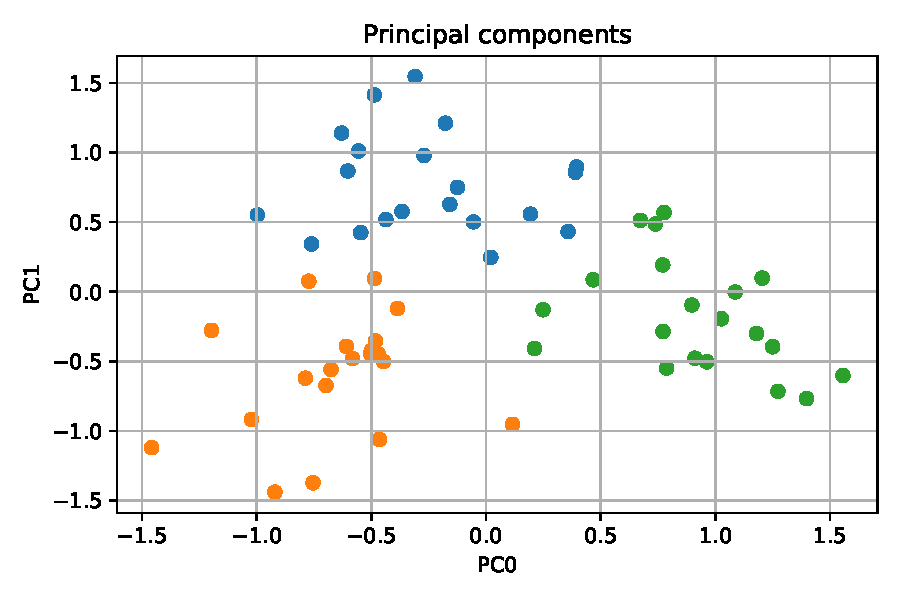
\includegraphics[width = 0.6\textwidth]{3-pca}
    \caption{Primeras dos componentes principales para las 60 observaciones generadas. Cada color representa que son de un grupo distinto}
    \label{3-pca}
\end{figure}
En la figura podemos observar que las observaciones se separan en los tres grupos de manera muy clara en el espacio de las componentes principales.
\subsection{Incisos c), d), e) y g)}
Pretendemos ahora usar el algoritmo de $K$-means para realizar clustering sobre las observaciones originales, estandarizadas y con desviación estándar 1 para $K=3,2,4$. Presentamos los resultados de dicho clustering graficando las tres primeras componentes de los vectores $Z_i$ y marcando clusters distintos con colores distintos.
\\
\\La tabla \ref{3-clusresults} muestra que con los datos originales la separación en grupos originales siempre se logra, a excepción de uno o dos puntos, para $K=3$. Para $K=2$, dos de estos grupos se fusionan, mientras que para $K=4$ un grupo se separa en dos y dos de los originales se  mantienen relativamente bien.
\\
\\Un comportamiento parecido se obtiene cuando hacemos que los datos tengan $\sigma^2 = 1$, aunque con menor calidad en los resultados. Sin embargo, si estandarizamos los datos, el algoritmo deja de distinguir los grupos. La explicación a esto es clara, ya que por la construcción de los datos, lo que diferencía a cada grupo es una constante que se suma, que se quita de todos cuando le quitamos el valor promedio, por lo que los datos vuelven a su distribución aleatoria y no existe una distinción clara entre ellos.
\subsection{Inciso f)}
Las gráficas \ref{3-2pcs-2}, \ref{3-2pcs-3} y \ref{3-2pcs-4} muestran los resultados de aplicar el clustering sobre las dos primeras componentes principales para $K=3,4,2$, mientrasl que la tabla \ref{3-clusresults-pca}. Para $K=3$ la separación se logra de manera normal y óptima, mientras que para $K=2$ dos grupos se fusionan en uno y para $K=4$ los grupos uno y dos se dividen en tres grupos.
\section{Ejercicio 11}
Dato un conjunto de 40 tejidos que son representados por 1000 genes, sabemos a priori que los 20 primeros tejidos son muestras sanas mientras que los últimos 20 genes son de tejido enfermo. 
\subsection{Inciso b)}
Queremos aplicar clustering jerárquico a los datos usando distancia basada en correlación para separarlos en dos grupos. El dendrograma resultante para las 9 combinaciones de los datos originales, estandarizados y con $\sigma^2 = 1$ y para los tres tipos de enlace entre clusters se muestran en las figuras \ref{4-completeoriginal}, \ref{4-completestandarized}, \ref{4-completewithmean}, \ref{4-singleoriginal}, \ref{4-singlestandarized}, \ref{4-singlewithmean}, \ref{4-averageoriginal}, \ref{4-averagestandarized} y  \ref{4-averagewithmean}.
\\
\\Para la tabla \ref{4-clusres} muestra el etiquetado obtenido a partir de estos algoritmos. Como podemos ver, los únicos datos en los cuales el clutering jerárquico si logra dividirlos en los dos grupos conocidos es para los datos estandarizados. Para los tipos de datos, el resultado varia según el tipo de enlace pero en general podemos afirmar que no  se separan en los grupos buscados o en un caso (enlace promedio y datos con $\sigma^2 = 1$) no hay dos grupos pues un tejido termina siendo su propio cluster.
\\
\\Notemos que, para los datos estandarizados, la separación en los dos grupos conocidos se cumple para cualquier enlace entre clusters, es decir, es independiente del enlace. Podemos concluir que, para este conjunto de datos, la estandarización si resulta necesaria para obtener resultados satisfactorios.
\subsection{Inciso c)}
Queremos ahora determinar cual es el conjunto de genes que difieren más entre ambos grupos. Claramente no hay una manera axiomática de resolver este problema, por lo presentamos tres métodos utilizados para abordar dicho poblema.
\subsubsection{Método 1: maximizar la norma de la matriz de diferencias}
Para cada gen $k$, definimos la matriz de diferencias $A^{(k)}$ de la siguiente forma
\begin{equation}
    A^{(k)}_{ij} = x_{ik} - x_{jk}
\end{equation}
Es decir, $A^{(k)}_{ij}$ es la diferencia del valor del gen $k$ entre los tejidos $i,j$. Recordando que la norma de Frobenius de una matriz $D$ de $n \times m$ es
\begin{equation}
    |D| = \sqrt{ \sum_{i=1}^{n} \sum_{j=1}^{m} |D_{ij}|^2 }
\end{equation}
Es claro que la norma de Frobenius de la matriz $A^{(k)}$ cuantifica cuanto varían las observaciones entre ambos grupos. Así, podemos decir entonces que los genes con mayor variación son aquellos cuya matriz de variación es máxima. La tabla \ref{4-variance-distance} en el Anexo 1 presenta cuales son los 20 genes que maximizan dicho valor. 
\subsubsection{Método 2: quitar un subconjunto de genes y ver si el clustering se logra}
En principio, el conjunto de variables que varía más es el conjunto de genes tales que al removerlos de los datos de los tejidos e intentar hacer clustering jerárquico sobre los genes restantes, este no divide a los tejidos en los dos grupos conocidos.
\\
\\Sabemos que hay $\frac{1000!}{n!(1000-n)!}$ subconjuntos de $n$ genes, por lo que es muy complicado ir probando con todos los subconjuntos de distintos tamaños para utilizar este método. Sin embargo, una manera más simple sería empezar simplemente remover un gen del conjunto de datos y ver si el clustering se logra.
\\
\\Se implementó dicho procedimiento en el código y lo que se obtuvo, en principio, es que solo removiendo un gen de los datos, de igual manera se logra hacer el clustering jerárquico para los tres tipos de enlace, por lo que este método no nos resulta satisfactorio quitando solo un gen.
\\
\\Por el tiempo de cómputo, no se intentó realizar la prueba quitando subconjuntos de más de un gen.
\subsubsection{Método 3: intentar hacer clustering con solo un subconjunto de genes}
Pensando el problema de manera inversa al método anterior, podríamos pensar que si logramos realizar el clustering en los dos grupos conocidos utilizando un subconjunto mínimo de genes, esos son los que permiten distinguirlos en ambos grupos y los que varían más. Nuevamente, por el número de subconjuntos, esto no es práctico.
\\
\\Nos limitamos a analizar el clustering utilizando solamente un gen y ver si era posible diferenciarlos en los grupos buscados. No resultó posible hacer dicha separación con un solo gen de manera perfecta. Sin embargo, podemos cuantificar, con la ecuación \ref{erroratio}, la razón de errores de cada clasificación con un solo gen:
\begin{equation}
    \label{erroratio}
    \text{error} = \frac{N_{\text{aciertos}}}{N_{tejidos}}
\end{equation}
La tabla \ref{4-errors-ratio} en el Anexo 1 presenta cuales son los 20 genes que maximizan dicho valor para distintos tipos de enlace
\subsubsection{Conclusiones}
Al comprar los genes obtenidos por los métodos 1 y 3, es claro que el conjunto de genes contiene varios en común. En particular, el gen 501 aparece como el más variante en ambos métodos.
\\
\\Debido a esta coincidencia en resultados, consideramos que los resultados arrojados por ambos métodos son satisfactorios.
\\
\\
Además, notemos que el haber tomado 20 genes fue arbitario. En general, podríamos usarlos para ordenar los genes según su variación.
\pagebreak
\section*{Anexo 1: Tablas relevantes}
\subsection*{Resultados del clustering para el ejercicio 9}
\begin{longtable}{cp{1.5cm}p{1.5cm}p{1.5cm}p{1.5cm}p{1.5cm}p{1.5cm}p{1.5cm}p{1.5cm}p{1.5cm}}
\toprule
{} &  Cluster complete original &  Cluster complete standarized &  Cluster complete withmean &  Cluster single original &  Cluster single standarized &  Cluster single withmean &  Cluster average original &  Cluster average standarized &  Cluster average withmean \\
\midrule
\endhead
\midrule
\multicolumn{10}{r}{{Continued on next page}} \\
\midrule
\endfoot

\bottomrule
\endlastfoot
Alabama &                          0 &                             0 &                          0 &                        0 &                           0 &                        0 &                         0 &                            0 &                         0 \\
Alaska  &                          0 &                             0 &                          0 &                        0 &                           1 &                        1 &                         0 &                            2 &                         2 \\
Arizona &                          0 &                             1 &                          1 &                        0 &                           0 &                        0 &                         0 &                            0 &                         0 \\
Arkansa &                          2 &                             2 &                          2 &                        0 &                           0 &                        0 &                         2 &                            1 &                         1 \\
Califor &                          0 &                             1 &                          1 &                        0 &                           0 &                        0 &                         0 &                            0 &                         0 \\
Colorad &                          2 &                             1 &                          1 &                        0 &                           0 &                        0 &                         2 &                            0 &                         0 \\
Connect &                          1 &                             2 &                          2 &                        0 &                           0 &                        0 &                         1 &                            1 &                         1 \\
Delawar &                          0 &                             2 &                          2 &                        0 &                           0 &                        0 &                         0 &                            1 &                         1 \\
Florida &                          0 &                             1 &                          1 &                        2 &                           2 &                        2 &                         0 &                            0 &                         0 \\
Georgia &                          2 &                             0 &                          0 &                        0 &                           0 &                        0 &                         2 &                            0 &                         0 \\
Hawaii  &                          1 &                             2 &                          2 &                        0 &                           0 &                        0 &                         1 &                            1 &                         1 \\
Idaho   &                          1 &                             2 &                          2 &                        0 &                           0 &                        0 &                         1 &                            1 &                         1 \\
Illinoi &                          0 &                             1 &                          1 &                        0 &                           0 &                        0 &                         0 &                            0 &                         0 \\
Indiana &                          1 &                             2 &                          2 &                        0 &                           0 &                        0 &                         1 &                            1 &                         1 \\
Iowa    &                          1 &                             2 &                          2 &                        0 &                           0 &                        0 &                         1 &                            1 &                         1 \\
Kansas  &                          1 &                             2 &                          2 &                        0 &                           0 &                        0 &                         1 &                            1 &                         1 \\
Kentuck &                          1 &                             2 &                          2 &                        0 &                           0 &                        0 &                         1 &                            1 &                         1 \\
Louisia &                          0 &                             0 &                          0 &                        0 &                           0 &                        0 &                         0 &                            0 &                         0 \\
Maine   &                          1 &                             2 &                          2 &                        0 &                           0 &                        0 &                         1 &                            1 &                         1 \\
Marylan &                          0 &                             1 &                          1 &                        0 &                           0 &                        0 &                         0 &                            0 &                         0 \\
Massach &                          2 &                             2 &                          2 &                        0 &                           0 &                        0 &                         2 &                            1 &                         1 \\
Michiga &                          0 &                             1 &                          1 &                        0 &                           0 &                        0 &                         0 &                            0 &                         0 \\
Minneso &                          1 &                             2 &                          2 &                        0 &                           0 &                        0 &                         1 &                            1 &                         1 \\
Mississ &                          0 &                             0 &                          0 &                        0 &                           0 &                        0 &                         0 &                            0 &                         0 \\
Missour &                          2 &                             2 &                          2 &                        0 &                           0 &                        0 &                         2 &                            0 &                         0 \\
Montana &                          1 &                             2 &                          2 &                        0 &                           0 &                        0 &                         1 &                            1 &                         1 \\
Nebrask &                          1 &                             2 &                          2 &                        0 &                           0 &                        0 &                         1 &                            1 &                         1 \\
Nevada  &                          0 &                             1 &                          1 &                        0 &                           0 &                        0 &                         0 &                            0 &                         0 \\
New Ham &                          1 &                             2 &                          2 &                        0 &                           0 &                        0 &                         1 &                            1 &                         1 \\
New Jer &                          2 &                             2 &                          2 &                        0 &                           0 &                        0 &                         2 &                            1 &                         1 \\
New Mex &                          0 &                             1 &                          1 &                        0 &                           0 &                        0 &                         0 &                            0 &                         0 \\
New Yor &                          0 &                             1 &                          1 &                        0 &                           0 &                        0 &                         0 &                            0 &                         0 \\
North C &                          0 &                             0 &                          0 &                        1 &                           0 &                        0 &                         0 &                            0 &                         0 \\
North D &                          1 &                             2 &                          2 &                        0 &                           0 &                        0 &                         1 &                            1 &                         1 \\
Ohio    &                          1 &                             2 &                          2 &                        0 &                           0 &                        0 &                         1 &                            1 &                         1 \\
Oklahom &                          2 &                             2 &                          2 &                        0 &                           0 &                        0 &                         2 &                            1 &                         1 \\
Oregon  &                          2 &                             2 &                          2 &                        0 &                           0 &                        0 &                         2 &                            1 &                         1 \\
Pennsyl &                          1 &                             2 &                          2 &                        0 &                           0 &                        0 &                         1 &                            1 &                         1 \\
Rhode I &                          2 &                             2 &                          2 &                        0 &                           0 &                        0 &                         2 &                            1 &                         1 \\
South C &                          0 &                             0 &                          0 &                        0 &                           0 &                        0 &                         0 &                            0 &                         0 \\
South D &                          1 &                             2 &                          2 &                        0 &                           0 &                        0 &                         1 &                            1 &                         1 \\
Tenness &                          2 &                             0 &                          0 &                        0 &                           0 &                        0 &                         2 &                            0 &                         0 \\
Texas   &                          2 &                             1 &                          1 &                        0 &                           0 &                        0 &                         2 &                            0 &                         0 \\
Utah    &                          1 &                             2 &                          2 &                        0 &                           0 &                        0 &                         1 &                            1 &                         1 \\
Vermont &                          1 &                             2 &                          2 &                        0 &                           0 &                        0 &                         1 &                            1 &                         1 \\
Virgini &                          2 &                             2 &                          2 &                        0 &                           0 &                        0 &                         2 &                            1 &                         1 \\
Washing &                          2 &                             2 &                          2 &                        0 &                           0 &                        0 &                         2 &                            1 &                         1 \\
West Vi &                          1 &                             2 &                          2 &                        0 &                           0 &                        0 &                         1 &                            1 &                         1 \\
Wiscons &                          1 &                             2 &                          2 &                        0 &                           0 &                        0 &                         1 &                            1 &                         1 \\
Wyoming &                          2 &                             2 &                          2 &                        0 &                           0 &                        0 &                         2 &                            1 &                         1 \\
\end{longtable}

\begin{table}[H]
    \centering
    \centering
    \caption{Resultados de clustering con distintas escalas en los datos y distintos tipos de enlace}
    \label{2-clusresults}
\end{table}
\subsection*{Resultados del clustering para el ejercicio 10}
\begin{longtable}{cp{1.5cm}p{1.5cm}p{1.5cm}p{1.5cm}p{1.5cm}p{1.5cm}p{1.5cm}p{1.5cm}p{1.5cm}}
\toprule
{} &  K: 3 , data: original &  K: 2 , data: original &  K: 4 , data: original &  K: 3 , data: standarized &  K: 2 , data: standarized &  K: 4 , data: standarized &  K: 3 , data: withmean &  K: 2 , data: withmean &  K: 4 , data: withmean \\
\midrule
\endhead
\midrule
\multicolumn{10}{r}{{Continued on next page}} \\
\midrule
\endfoot

\bottomrule
\endlastfoot
0  &                      0 &                      0 &                      0 &                         0 &                         0 &                         0 &                      0 &                      0 &                      0 \\
1  &                      0 &                      1 &                      0 &                         2 &                         1 &                         1 &                      1 &                      1 &                      0 \\
2  &                      0 &                      1 &                      0 &                         2 &                         1 &                         3 &                      2 &                      0 &                      3 \\
3  &                      0 &                      0 &                      0 &                         0 &                         0 &                         0 &                      2 &                      0 &                      2 \\
4  &                      0 &                      1 &                      0 &                         2 &                         1 &                         3 &                      0 &                      1 &                      0 \\
5  &                      0 &                      1 &                      0 &                         0 &                         0 &                         0 &                      0 &                      0 &                      2 \\
6  &                      0 &                      1 &                      0 &                         1 &                         1 &                         3 &                      0 &                      1 &                      1 \\
7  &                      0 &                      1 &                      0 &                         0 &                         0 &                         2 &                      1 &                      1 &                      2 \\
8  &                      0 &                      1 &                      0 &                         2 &                         0 &                         3 &                      1 &                      0 &                      0 \\
9  &                      0 &                      1 &                      2 &                         2 &                         1 &                         3 &                      0 &                      0 &                      1 \\
10 &                      0 &                      1 &                      0 &                         2 &                         1 &                         1 &                      1 &                      1 &                      0 \\
11 &                      0 &                      1 &                      0 &                         2 &                         1 &                         0 &                      1 &                      0 &                      0 \\
12 &                      0 &                      0 &                      0 &                         0 &                         0 &                         2 &                      2 &                      0 &                      2 \\
13 &                      0 &                      1 &                      0 &                         2 &                         0 &                         0 &                      1 &                      1 &                      0 \\
14 &                      0 &                      1 &                      0 &                         2 &                         0 &                         0 &                      2 &                      0 &                      0 \\
15 &                      0 &                      0 &                      0 &                         0 &                         0 &                         0 &                      2 &                      0 &                      2 \\
16 &                      0 &                      1 &                      0 &                         1 &                         1 &                         0 &                      0 &                      1 &                      0 \\
17 &                      0 &                      1 &                      0 &                         2 &                         1 &                         1 &                      1 &                      1 &                      0 \\
18 &                      0 &                      1 &                      0 &                         1 &                         1 &                         1 &                      1 &                      1 &                      1 \\
19 &                      0 &                      1 &                      0 &                         0 &                         1 &                         2 &                      0 &                      0 &                      3 \\
20 &                      1 &                      1 &                      2 &                         2 &                         1 &                         1 &                      1 &                      1 &                      0 \\
21 &                      1 &                      1 &                      3 &                         2 &                         1 &                         2 &                      0 &                      0 &                      3 \\
22 &                      1 &                      1 &                      3 &                         2 &                         1 &                         3 &                      2 &                      0 &                      3 \\
23 &                      1 &                      1 &                      2 &                         0 &                         1 &                         2 &                      0 &                      0 &                      1 \\
24 &                      1 &                      0 &                      3 &                         0 &                         0 &                         2 &                      2 &                      0 &                      2 \\
25 &                      1 &                      1 &                      2 &                         2 &                         1 &                         3 &                      0 &                      0 &                      1 \\
26 &                      1 &                      1 &                      3 &                         1 &                         1 &                         2 &                      0 &                      0 &                      1 \\
27 &                      1 &                      1 &                      2 &                         1 &                         1 &                         2 &                      0 &                      1 &                      1 \\
28 &                      1 &                      1 &                      3 &                         1 &                         1 &                         3 &                      2 &                      0 &                      3 \\
29 &                      1 &                      1 &                      2 &                         1 &                         1 &                         2 &                      0 &                      1 &                      1 \\
30 &                      1 &                      1 &                      2 &                         2 &                         1 &                         0 &                      0 &                      1 &                      0 \\
31 &                      1 &                      1 &                      3 &                         0 &                         1 &                         2 &                      2 &                      0 &                      1 \\
32 &                      1 &                      1 &                      2 &                         1 &                         1 &                         3 &                      0 &                      1 &                      3 \\
33 &                      1 &                      1 &                      2 &                         0 &                         1 &                         2 &                      0 &                      1 &                      1 \\
34 &                      1 &                      1 &                      2 &                         1 &                         1 &                         1 &                      0 &                      1 &                      1 \\
35 &                      1 &                      1 &                      3 &                         2 &                         1 &                         0 &                      2 &                      0 &                      3 \\
36 &                      1 &                      1 &                      3 &                         1 &                         1 &                         0 &                      0 &                      0 &                      3 \\
37 &                      1 &                      1 &                      2 &                         0 &                         0 &                         2 &                      0 &                      0 &                      2 \\
38 &                      1 &                      1 &                      2 &                         0 &                         1 &                         0 &                      0 &                      0 &                      1 \\
39 &                      1 &                      1 &                      3 &                         0 &                         0 &                         2 &                      2 &                      0 &                      3 \\
40 &                      2 &                      0 &                      1 &                         0 &                         0 &                         2 &                      2 &                      0 &                      2 \\
41 &                      2 &                      0 &                      1 &                         2 &                         0 &                         1 &                      1 &                      0 &                      1 \\
42 &                      2 &                      0 &                      1 &                         0 &                         0 &                         2 &                      0 &                      1 &                      2 \\
43 &                      2 &                      0 &                      1 &                         1 &                         0 &                         3 &                      2 &                      0 &                      1 \\
44 &                      2 &                      0 &                      1 &                         1 &                         0 &                         3 &                      2 &                      0 &                      1 \\
45 &                      2 &                      0 &                      1 &                         0 &                         0 &                         2 &                      0 &                      1 &                      2 \\
46 &                      2 &                      0 &                      1 &                         1 &                         1 &                         1 &                      0 &                      1 &                      0 \\
47 &                      2 &                      0 &                      1 &                         1 &                         1 &                         1 &                      1 &                      1 &                      1 \\
48 &                      2 &                      0 &                      1 &                         2 &                         0 &                         1 &                      1 &                      1 &                      0 \\
49 &                      2 &                      0 &                      1 &                         0 &                         0 &                         0 &                      2 &                      0 &                      2 \\
50 &                      2 &                      0 &                      1 &                         2 &                         0 &                         3 &                      2 &                      0 &                      3 \\
51 &                      2 &                      1 &                      1 &                         2 &                         1 &                         3 &                      2 &                      0 &                      3 \\
52 &                      2 &                      0 &                      1 &                         1 &                         1 &                         3 &                      0 &                      1 &                      1 \\
53 &                      2 &                      1 &                      2 &                         2 &                         0 &                         1 &                      1 &                      1 &                      0 \\
54 &                      2 &                      0 &                      1 &                         1 &                         1 &                         3 &                      2 &                      0 &                      3 \\
55 &                      2 &                      0 &                      1 &                         1 &                         1 &                         3 &                      0 &                      1 &                      1 \\
56 &                      2 &                      0 &                      1 &                         0 &                         0 &                         2 &                      2 &                      0 &                      2 \\
57 &                      2 &                      0 &                      1 &                         2 &                         0 &                         3 &                      1 &                      1 &                      0 \\
58 &                      2 &                      0 &                      1 &                         1 &                         1 &                         3 &                      2 &                      0 &                      1 \\
59 &                      2 &                      0 &                      1 &                         0 &                         0 &                         3 &                      2 &                      0 &                      3 \\
\end{longtable}

\begin{table}[H]
    \centering
    \centering
    \caption{Resultados de clustering con $K$-means para datos originales, estandarizados y con $\sigma^2 = 1$ para distintos $K$}
    \label{3-clusresults}
\end{table}
\begin{longtable}{cp{3cm}p{3cm}p{3cm}}
\toprule
{} &  data: pca 2 vars, K=3 &  data: pca 2 vars, K=2 &  data: pca 2 vars, K=4 \\
\midrule
\endhead
\midrule
\multicolumn{4}{r}{{Continued on next page}} \\
\midrule
\endfoot

\bottomrule
\endlastfoot
0  &                      0 &                      0 &                      0 \\
1  &                      0 &                      1 &                      3 \\
2  &                      0 &                      1 &                      3 \\
3  &                      0 &                      0 &                      0 \\
4  &                      0 &                      1 &                      3 \\
5  &                      0 &                      1 &                      3 \\
6  &                      0 &                      1 &                      3 \\
7  &                      0 &                      1 &                      0 \\
8  &                      0 &                      1 &                      3 \\
9  &                      0 &                      1 &                      3 \\
10 &                      0 &                      1 &                      3 \\
11 &                      0 &                      1 &                      3 \\
12 &                      0 &                      0 &                      0 \\
13 &                      0 &                      1 &                      3 \\
14 &                      0 &                      1 &                      3 \\
15 &                      0 &                      0 &                      0 \\
16 &                      0 &                      1 &                      3 \\
17 &                      0 &                      1 &                      0 \\
18 &                      0 &                      1 &                      3 \\
19 &                      0 &                      1 &                      3 \\
20 &                      2 &                      1 &                      1 \\
21 &                      2 &                      1 &                      1 \\
22 &                      2 &                      1 &                      1 \\
23 &                      2 &                      1 &                      1 \\
24 &                      2 &                      0 &                      1 \\
25 &                      2 &                      1 &                      1 \\
26 &                      2 &                      1 &                      1 \\
27 &                      2 &                      1 &                      1 \\
28 &                      2 &                      1 &                      1 \\
29 &                      2 &                      1 &                      1 \\
30 &                      0 &                      1 &                      1 \\
31 &                      2 &                      1 &                      1 \\
32 &                      2 &                      1 &                      1 \\
33 &                      2 &                      1 &                      1 \\
34 &                      2 &                      1 &                      1 \\
35 &                      2 &                      1 &                      1 \\
36 &                      2 &                      1 &                      1 \\
37 &                      2 &                      1 &                      1 \\
38 &                      2 &                      1 &                      1 \\
39 &                      2 &                      1 &                      1 \\
40 &                      1 &                      0 &                      2 \\
41 &                      1 &                      0 &                      2 \\
42 &                      1 &                      0 &                      0 \\
43 &                      1 &                      0 &                      2 \\
44 &                      1 &                      0 &                      2 \\
45 &                      1 &                      0 &                      2 \\
46 &                      1 &                      0 &                      0 \\
47 &                      1 &                      0 &                      0 \\
48 &                      1 &                      0 &                      0 \\
49 &                      1 &                      0 &                      2 \\
50 &                      1 &                      0 &                      2 \\
51 &                      1 &                      0 &                      0 \\
52 &                      1 &                      0 &                      2 \\
53 &                      1 &                      0 &                      0 \\
54 &                      1 &                      0 &                      2 \\
55 &                      1 &                      0 &                      2 \\
56 &                      1 &                      0 &                      2 \\
57 &                      1 &                      0 &                      0 \\
58 &                      1 &                      0 &                      2 \\
59 &                      1 &                      0 &                      2 \\
\end{longtable}

\begin{table}[H]
    \centering
    \centering
    \caption{Resultados de clustering con $K$-means para las dos primeras componentes principales de los datos, estandarizados y con $\sigma^2 = 1$ para distintos $K$}
    \label{3-clusresults-pca}
\end{table}
\subsection*{Resultados del clustering para el ejercicio 11}
\begin{longtable}{cp{1.5cm}p{1.5cm}p{1.5cm}p{1.5cm}p{1.5cm}p{1.5cm}p{1.5cm}p{1.5cm}p{1.5cm}}
\toprule
{} &  Cluster complete original &  Cluster complete standarized &  Cluster complete withmean &  Cluster single original &  Cluster single standarized &  Cluster single withmean &  Cluster average original &  Cluster average standarized &  Cluster average withmean \\
\midrule
\endhead
\midrule
\multicolumn{10}{r}{{Continued on next page}} \\
\midrule
\endfoot

\bottomrule
\endlastfoot
0  &                          0 &                             0 &                          0 &                        0 &                           0 &                        0 &                         0 &                            0 &                         0 \\
1  &                          1 &                             0 &                          0 &                        0 &                           0 &                        1 &                         0 &                            0 &                         1 \\
2  &                          0 &                             0 &                          1 &                        0 &                           0 &                        1 &                         0 &                            0 &                         1 \\
3  &                          0 &                             0 &                          1 &                        0 &                           0 &                        1 &                         0 &                            0 &                         1 \\
4  &                          1 &                             0 &                          0 &                        0 &                           0 &                        1 &                         1 &                            0 &                         1 \\
5  &                          0 &                             0 &                          0 &                        0 &                           0 &                        1 &                         1 &                            0 &                         1 \\
6  &                          1 &                             0 &                          1 &                        0 &                           0 &                        1 &                         0 &                            0 &                         1 \\
7  &                          0 &                             0 &                          0 &                        0 &                           0 &                        1 &                         1 &                            0 &                         1 \\
8  &                          1 &                             0 &                          1 &                        0 &                           0 &                        1 &                         0 &                            0 &                         1 \\
9  &                          1 &                             0 &                          0 &                        0 &                           0 &                        1 &                         1 &                            0 &                         1 \\
10 &                          0 &                             0 &                          0 &                        0 &                           0 &                        1 &                         1 &                            0 &                         1 \\
11 &                          0 &                             0 &                          0 &                        0 &                           0 &                        1 &                         1 &                            0 &                         1 \\
12 &                          1 &                             0 &                          0 &                        0 &                           0 &                        1 &                         1 &                            0 &                         1 \\
13 &                          0 &                             0 &                          0 &                        0 &                           0 &                        1 &                         1 &                            0 &                         1 \\
14 &                          0 &                             0 &                          0 &                        0 &                           0 &                        1 &                         1 &                            0 &                         1 \\
15 &                          1 &                             0 &                          1 &                        0 &                           0 &                        1 &                         0 &                            0 &                         1 \\
16 &                          1 &                             0 &                          0 &                        0 &                           0 &                        1 &                         1 &                            0 &                         1 \\
17 &                          1 &                             0 &                          0 &                        0 &                           0 &                        1 &                         1 &                            0 &                         1 \\
18 &                          1 &                             0 &                          0 &                        1 &                           0 &                        1 &                         0 &                            0 &                         1 \\
19 &                          0 &                             0 &                          1 &                        0 &                           0 &                        1 &                         0 &                            0 &                         1 \\
20 &                          1 &                             1 &                          0 &                        0 &                           1 &                        1 &                         1 &                            1 &                         1 \\
21 &                          1 &                             1 &                          0 &                        0 &                           1 &                        1 &                         1 &                            1 &                         1 \\
22 &                          1 &                             1 &                          0 &                        0 &                           1 &                        1 &                         1 &                            1 &                         1 \\
23 &                          1 &                             1 &                          0 &                        0 &                           1 &                        1 &                         1 &                            1 &                         1 \\
24 &                          1 &                             1 &                          0 &                        0 &                           1 &                        1 &                         1 &                            1 &                         1 \\
25 &                          1 &                             1 &                          0 &                        0 &                           1 &                        1 &                         1 &                            1 &                         1 \\
26 &                          1 &                             1 &                          0 &                        0 &                           1 &                        1 &                         1 &                            1 &                         1 \\
27 &                          1 &                             1 &                          0 &                        0 &                           1 &                        1 &                         1 &                            1 &                         1 \\
28 &                          1 &                             1 &                          0 &                        0 &                           1 &                        1 &                         1 &                            1 &                         1 \\
29 &                          1 &                             1 &                          0 &                        0 &                           1 &                        1 &                         1 &                            1 &                         1 \\
30 &                          1 &                             1 &                          0 &                        0 &                           1 &                        1 &                         1 &                            1 &                         1 \\
31 &                          1 &                             1 &                          0 &                        0 &                           1 &                        1 &                         1 &                            1 &                         1 \\
32 &                          1 &                             1 &                          0 &                        0 &                           1 &                        1 &                         1 &                            1 &                         1 \\
33 &                          1 &                             1 &                          0 &                        0 &                           1 &                        1 &                         1 &                            1 &                         1 \\
34 &                          1 &                             1 &                          0 &                        0 &                           1 &                        1 &                         1 &                            1 &                         1 \\
35 &                          1 &                             1 &                          0 &                        0 &                           1 &                        1 &                         1 &                            1 &                         1 \\
36 &                          1 &                             1 &                          0 &                        0 &                           1 &                        1 &                         1 &                            1 &                         1 \\
37 &                          1 &                             1 &                          0 &                        0 &                           1 &                        1 &                         1 &                            1 &                         1 \\
38 &                          1 &                             1 &                          0 &                        0 &                           1 &                        1 &                         1 &                            1 &                         1 \\
39 &                          1 &                             1 &                          0 &                        0 &                           1 &                        1 &                         1 &                            1 &                         1 \\
\end{longtable}

\begin{table}[H]
    \centering
    \centering
    \caption{Resultados de clustering con distintas escalas en los datos y distintos tipos de enlace}
    \label{4-clusres}
\end{table}
\subsection*{Método 3 del inciso c) del ejercicio 11}
\begin{longtable}{cp{2cm}p{2cm}p{2cm}p{2cm}p{2cm}p{2cm}}
\toprule
{} &  original &  original variance distance &  standarized &  standarized variance distance &  withmean &  withmean variance distance \\
\midrule
\endhead
\midrule
\multicolumn{7}{r}{{Continued on next page}} \\
\midrule
\endfoot

\bottomrule
\endlastfoot
0  &       522 &                       54.29 &           10 &                          35.67 &        10 &                       35.67 \\
1  &       592 &                       54.73 &          591 &                          35.68 &       591 &                       35.68 \\
2  &       537 &                       54.88 &          554 &                          35.68 &       554 &                       35.68 \\
3  &       501 &                       55.25 &          569 &                          35.69 &       569 &                       35.69 \\
4  &       564 &                       55.36 &          539 &                          35.70 &       539 &                       35.70 \\
5  &       545 &                       55.79 &          510 &                          35.72 &       510 &                       35.72 \\
6  &       508 &                       55.85 &          534 &                          35.77 &       534 &                       35.77 \\
7  &       560 &                       55.90 &          553 &                          35.78 &       553 &                       35.78 \\
8  &       598 &                       56.09 &          507 &                          35.81 &       507 &                       35.81 \\
9  &       553 &                       56.25 &          563 &                          35.86 &       563 &                       35.86 \\
10 &        11 &                       56.34 &          568 &                          35.89 &       568 &                       35.89 \\
11 &       512 &                       56.64 &          537 &                          35.92 &       537 &                       35.92 \\
12 &       561 &                       57.82 &          583 &                          36.00 &       583 &                       36.00 \\
13 &       539 &                       58.98 &          592 &                          36.07 &       592 &                       36.07 \\
14 &       583 &                       59.48 &          550 &                          36.09 &       550 &                       36.09 \\
15 &       528 &                       59.99 &          564 &                          36.46 &       564 &                       36.46 \\
16 &       567 &                       60.07 &          589 &                          36.66 &       589 &                       36.66 \\
17 &       599 &                       60.33 &          599 &                          36.98 &       599 &                       36.98 \\
18 &       581 &                       60.39 &          588 &                          37.15 &       588 &                       37.15 \\
19 &       548 &                       60.57 &          501 &                          37.28 &       501 &                       37.28 \\
\end{longtable}

\begin{table}[H]
    \centering
    \centering
    \caption{Genes que minimizan la razón de errores}
    \label{4-variance-distance}
\end{table}
\subsection*{Método 3 del inciso c) del ejercicio 11}
\begin{longtable}{cp{2cm}p{2cm}p{2cm}p{2cm}p{2cm}p{2cm}}
\toprule
{} &  complete &  complete error ratio &  single &  single error ratio &  average &  average error ratio \\
\midrule
\endhead
\midrule
\multicolumn{7}{r}{{Continued on next page}} \\
\midrule
\endfoot

\bottomrule
\endlastfoot
0  &       501 &                 0.050 &     501 &               0.050 &      501 &                0.050 \\
1  &       550 &                 0.075 &     564 &               0.100 &      589 &                0.075 \\
2  &       589 &                 0.075 &     568 &               0.125 &      550 &                0.075 \\
3  &       565 &                 0.100 &      19 &               0.150 &      553 &                0.100 \\
4  &       569 &                 0.100 &     589 &               0.225 &      564 &                0.100 \\
5  &       592 &                 0.100 &     569 &               0.275 &      569 &                0.100 \\
6  &       548 &                 0.100 &     552 &               0.350 &      574 &                0.100 \\
7  &        12 &                 0.100 &      97 &               0.350 &      546 &                0.125 \\
8  &       529 &                 0.100 &     591 &               0.350 &      561 &                0.125 \\
9  &       546 &                 0.125 &     164 &               0.350 &      513 &                0.125 \\
10 &       553 &                 0.125 &      12 &               0.375 &      510 &                0.125 \\
11 &       544 &                 0.125 &     509 &               0.375 &      507 &                0.125 \\
12 &       561 &                 0.125 &      10 &               0.375 &      562 &                0.125 \\
13 &       535 &                 0.125 &     557 &               0.400 &      567 &                0.125 \\
14 &       587 &                 0.125 &     898 &               0.400 &      522 &                0.125 \\
15 &       586 &                 0.125 &     640 &               0.400 &      568 &                0.125 \\
16 &       507 &                 0.125 &     587 &               0.400 &      587 &                0.125 \\
17 &       567 &                 0.125 &     599 &               0.400 &      592 &                0.125 \\
18 &       568 &                 0.125 &     562 &               0.400 &      528 &                0.150 \\
19 &       513 &                 0.125 &     749 &               0.400 &      512 &                0.150 \\
\end{longtable}

\begin{table}[H]
    \centering
    \centering
    \caption{Genes que minimizan la razón de errores}
    \label{4-errors-ratio}
\end{table}
\section*{Anexo 2: Figuras relevantes}
\subsection*{Dendrogramas para el ejercicio 10}
\begin{figure}[H]
    \centering
    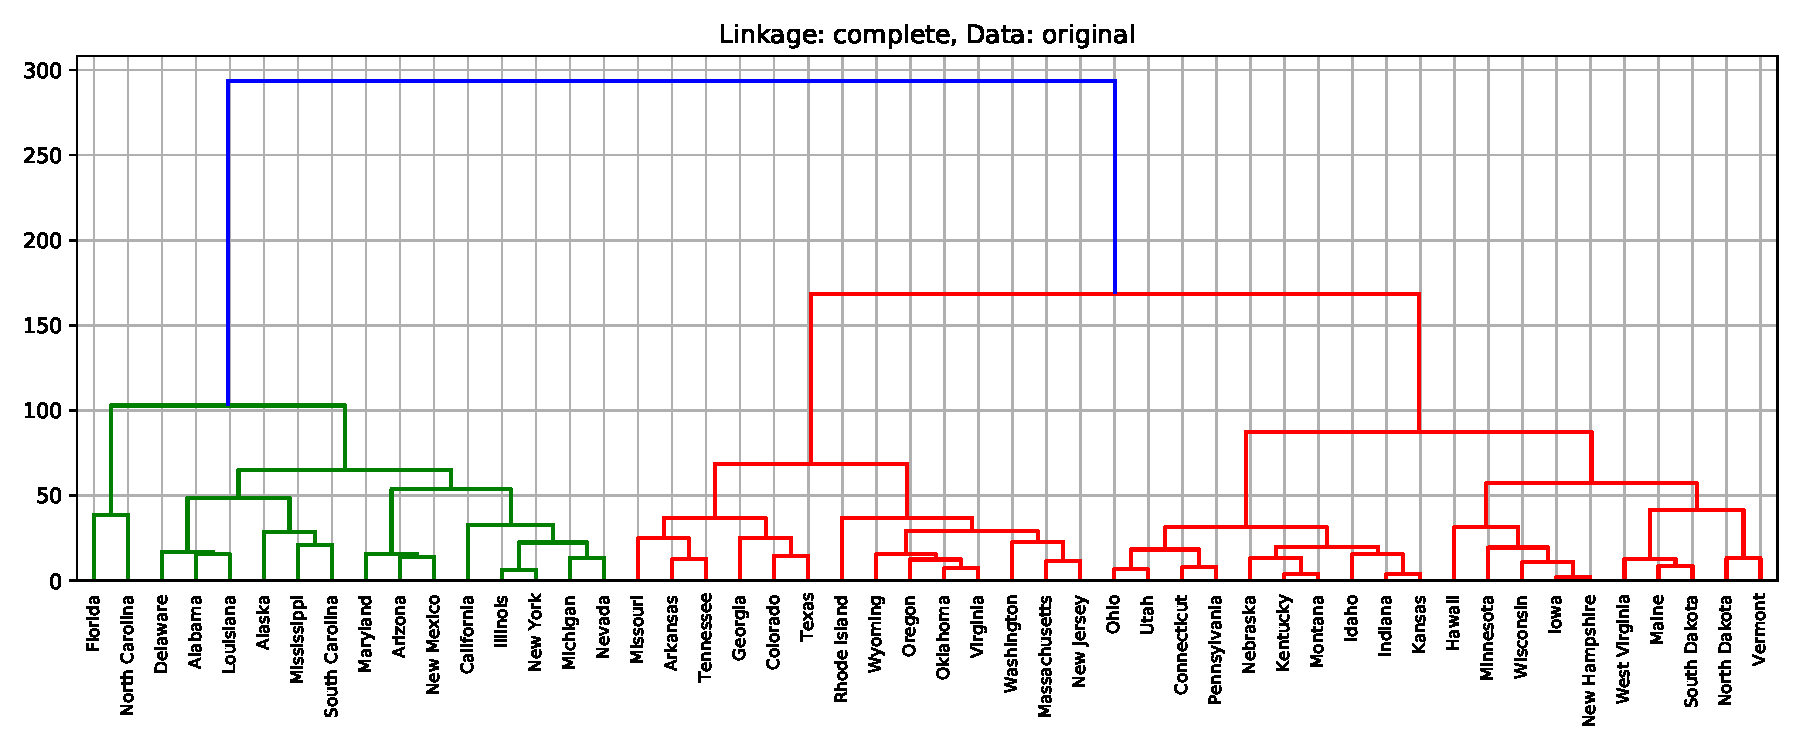
\includegraphics[width = 0.90\textwidth]{2-completeoriginal.pdf}
    \caption{Clustering para datos originales con enlace completo}
    \label{2-completeoriginal}
\end{figure}
\begin{figure}[H]
    \centering
    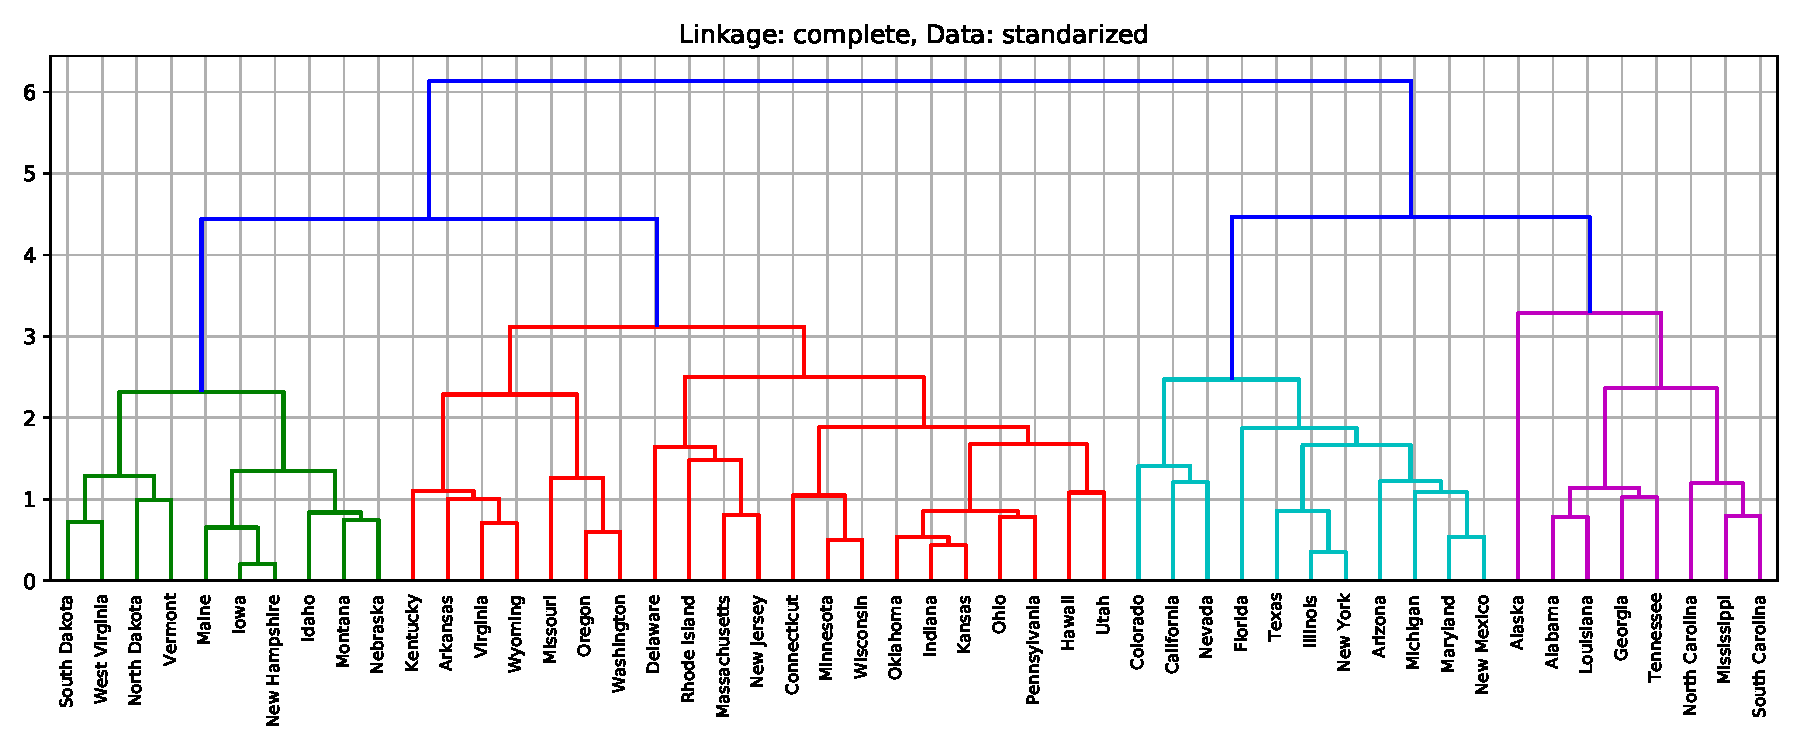
\includegraphics[width = 0.90\textwidth]{2-completestandarized.pdf}
    \caption{Clustering para datos estandarizados con enlace completo}
    \label{2-completestandarized}
\end{figure}
\begin{figure}[H]
    \centering
    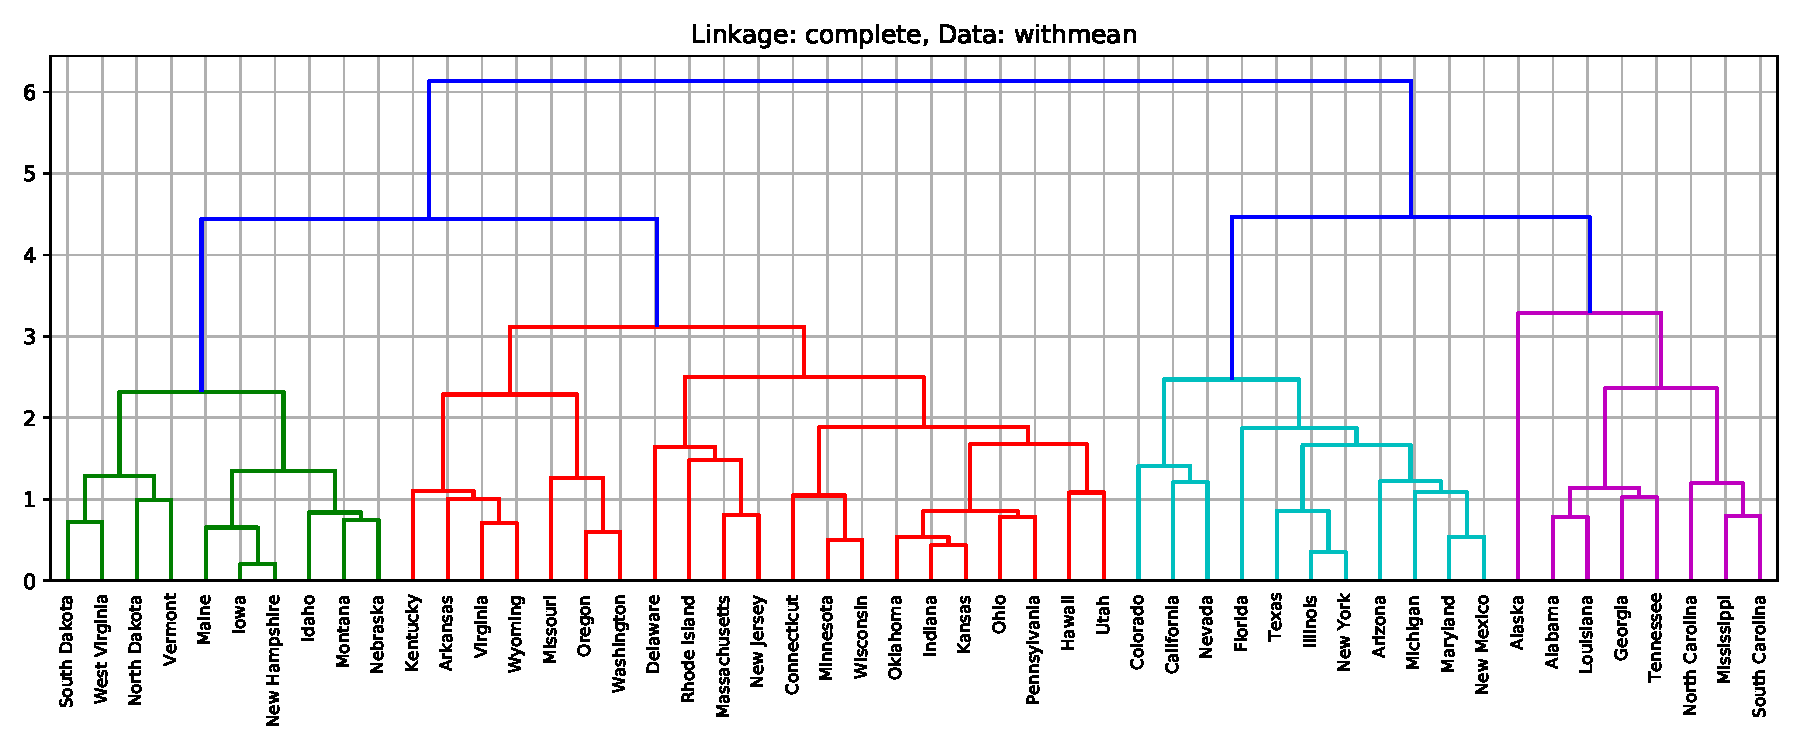
\includegraphics[width = 0.90\textwidth]{2-completewithmean.pdf}
    \caption{Clustering para datos con $\sigma^2 = 1$ con enlace completo}
    \label{2-completewithmean}
\end{figure}
\begin{figure}[H]
    \centering
    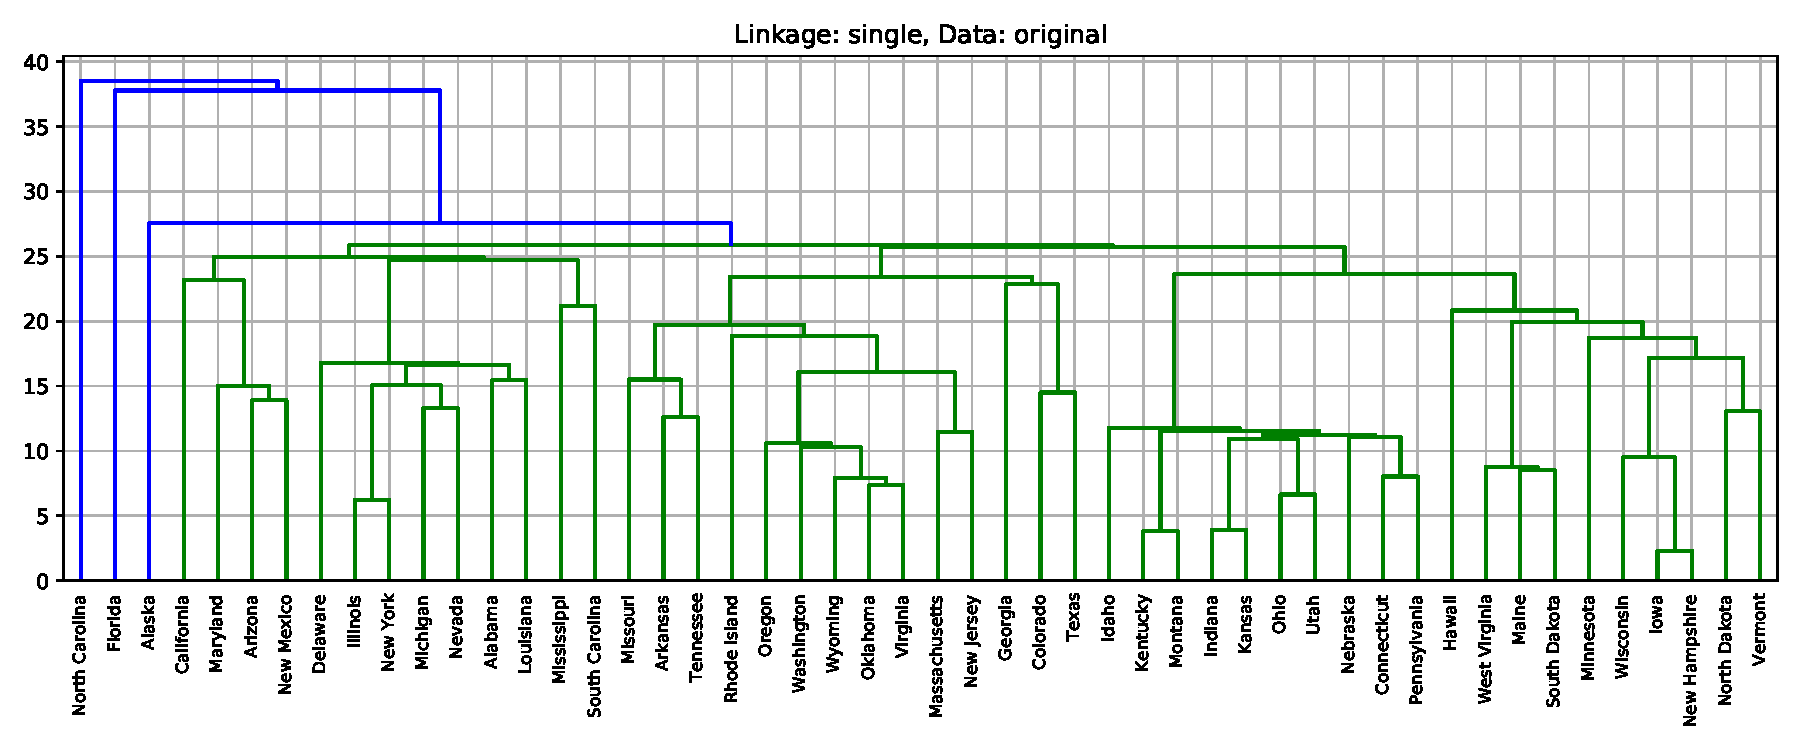
\includegraphics[width = 0.90\textwidth]{2-singleoriginal.pdf}
    \caption{Clustering para datos originales con enlace completo}
    \label{2-singleoriginal}
\end{figure}
\begin{figure}[H]
    \centering
    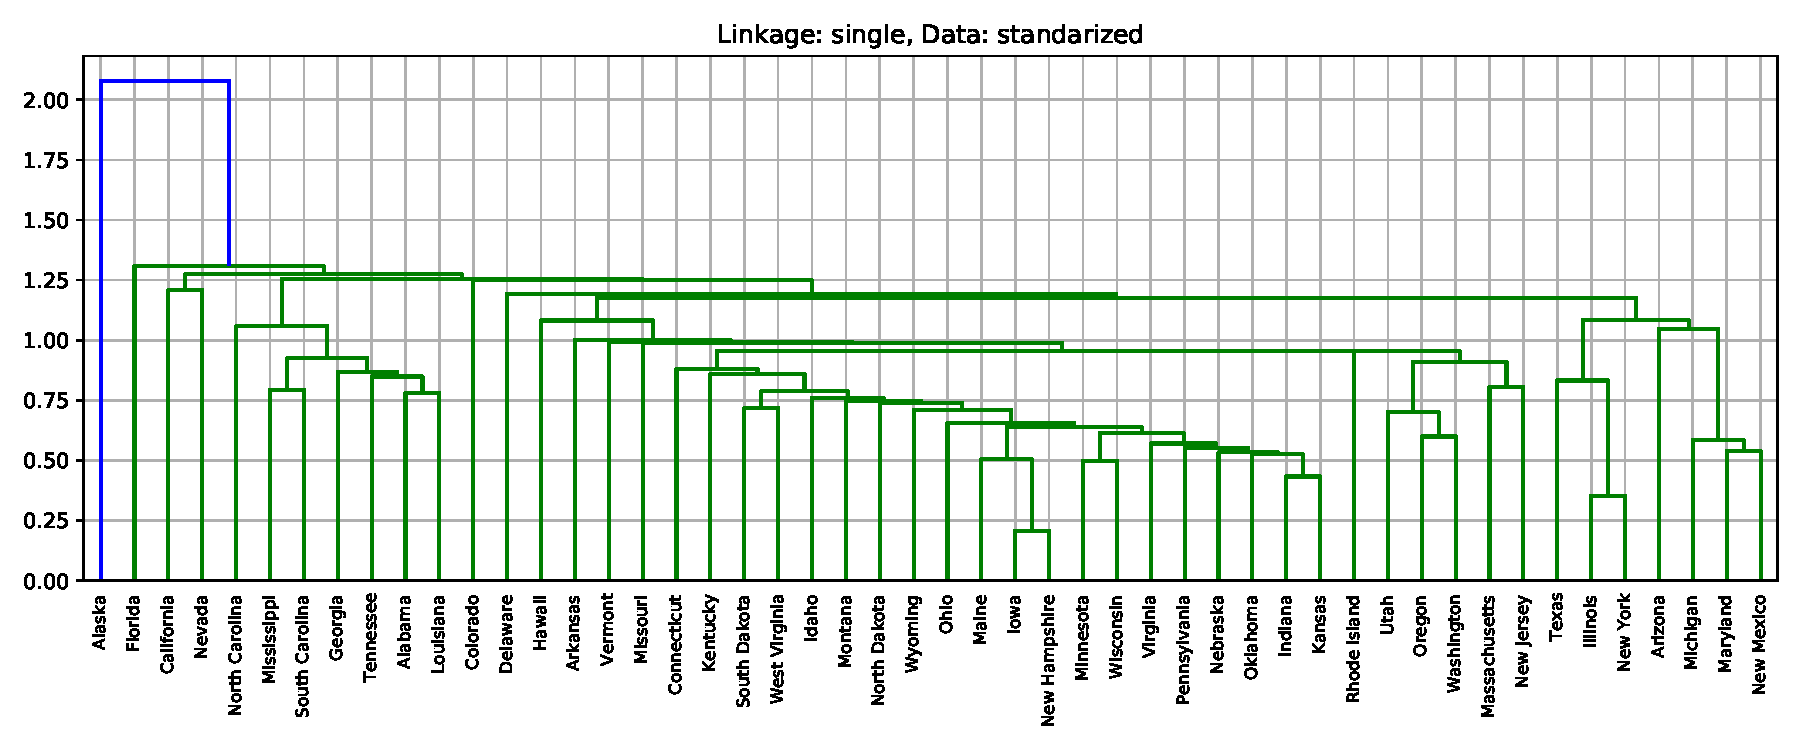
\includegraphics[width = 0.90\textwidth]{2-singlestandarized.pdf}
    \caption{Clustering para datos estandarizados con enlace completo}
    \label{2-singlestandarized}
\end{figure}
\begin{figure}[H]
    \centering
    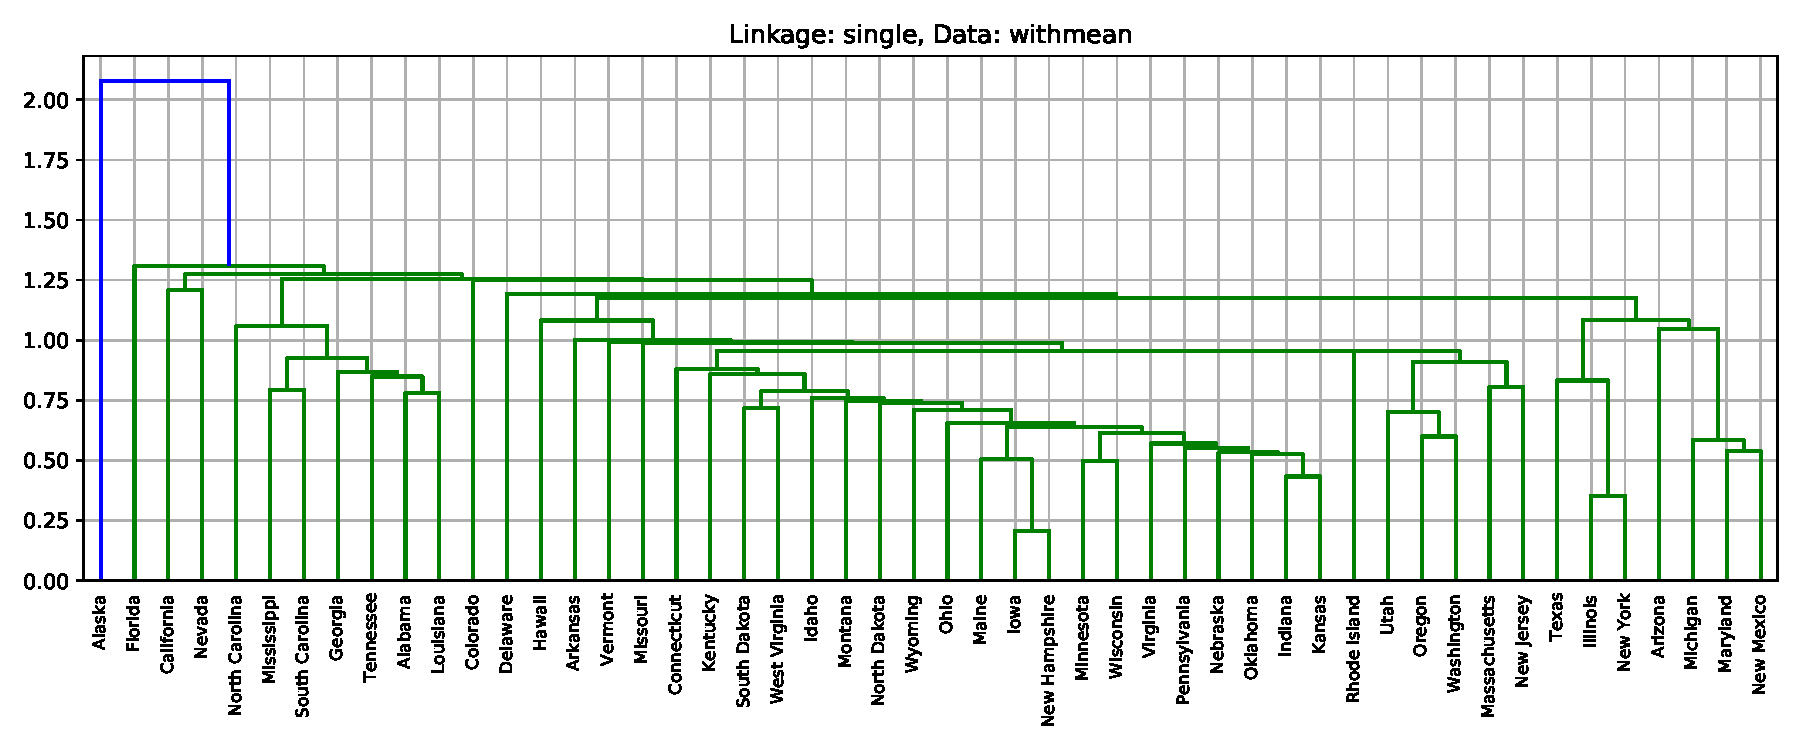
\includegraphics[width = 0.90\textwidth]{2-singlewithmean.pdf}
    \caption{Clustering para datos con $\sigma^2 = 1$ con enlace completo}
    \label{2-singlewithmean}
\end{figure}
\begin{figure}[H]
    \centering
    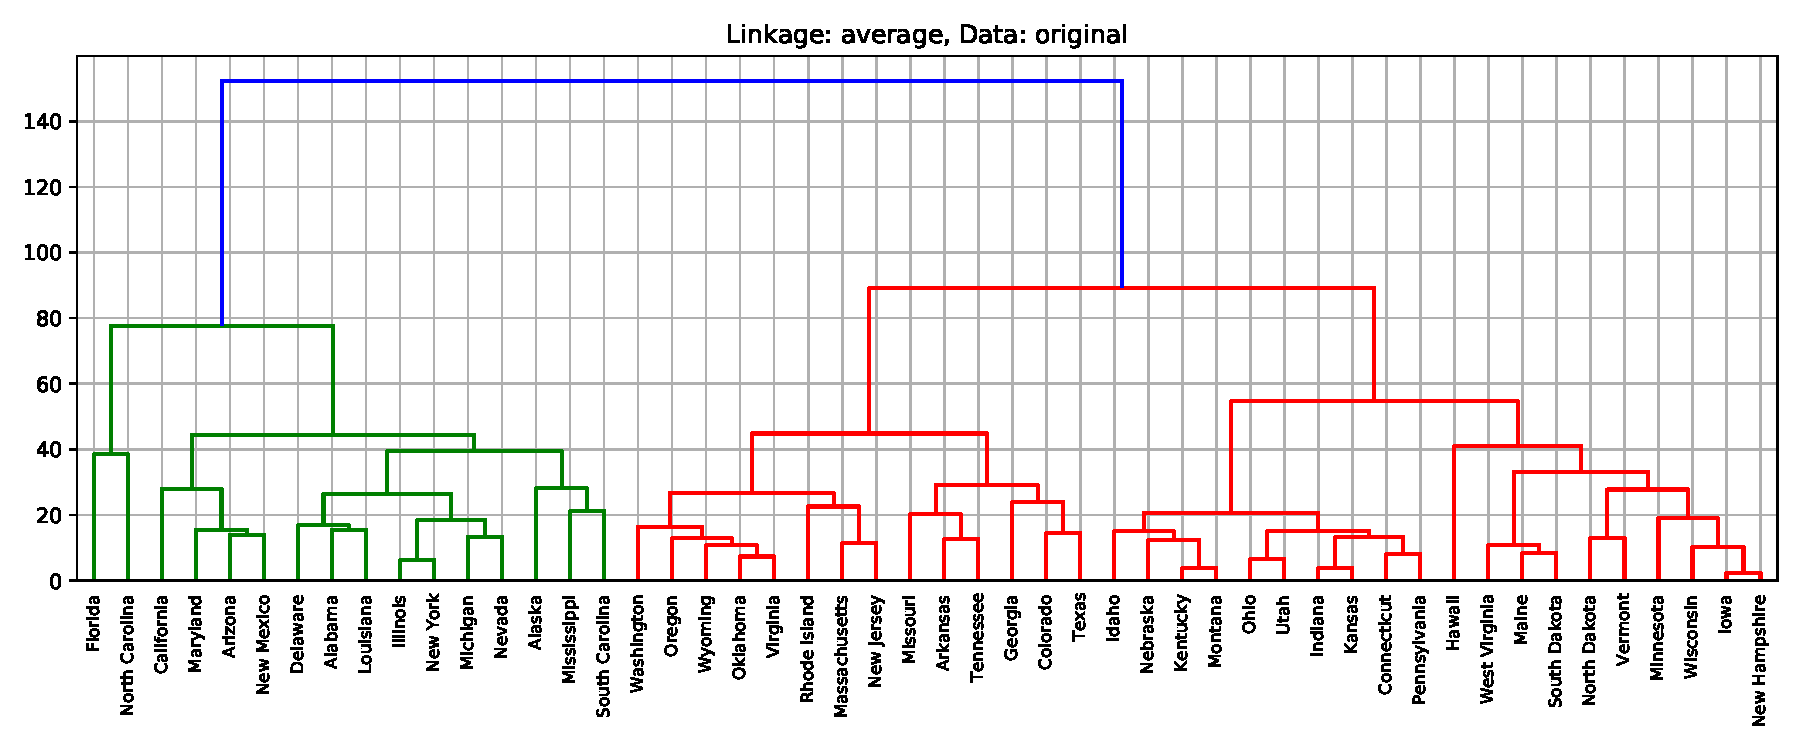
\includegraphics[width = 0.90\textwidth]{2-averageoriginal.pdf}
    \caption{Clustering para datos originales con enlace completo}
    \label{2-averageoriginal}
\end{figure}
\begin{figure}[H]
    \centering
    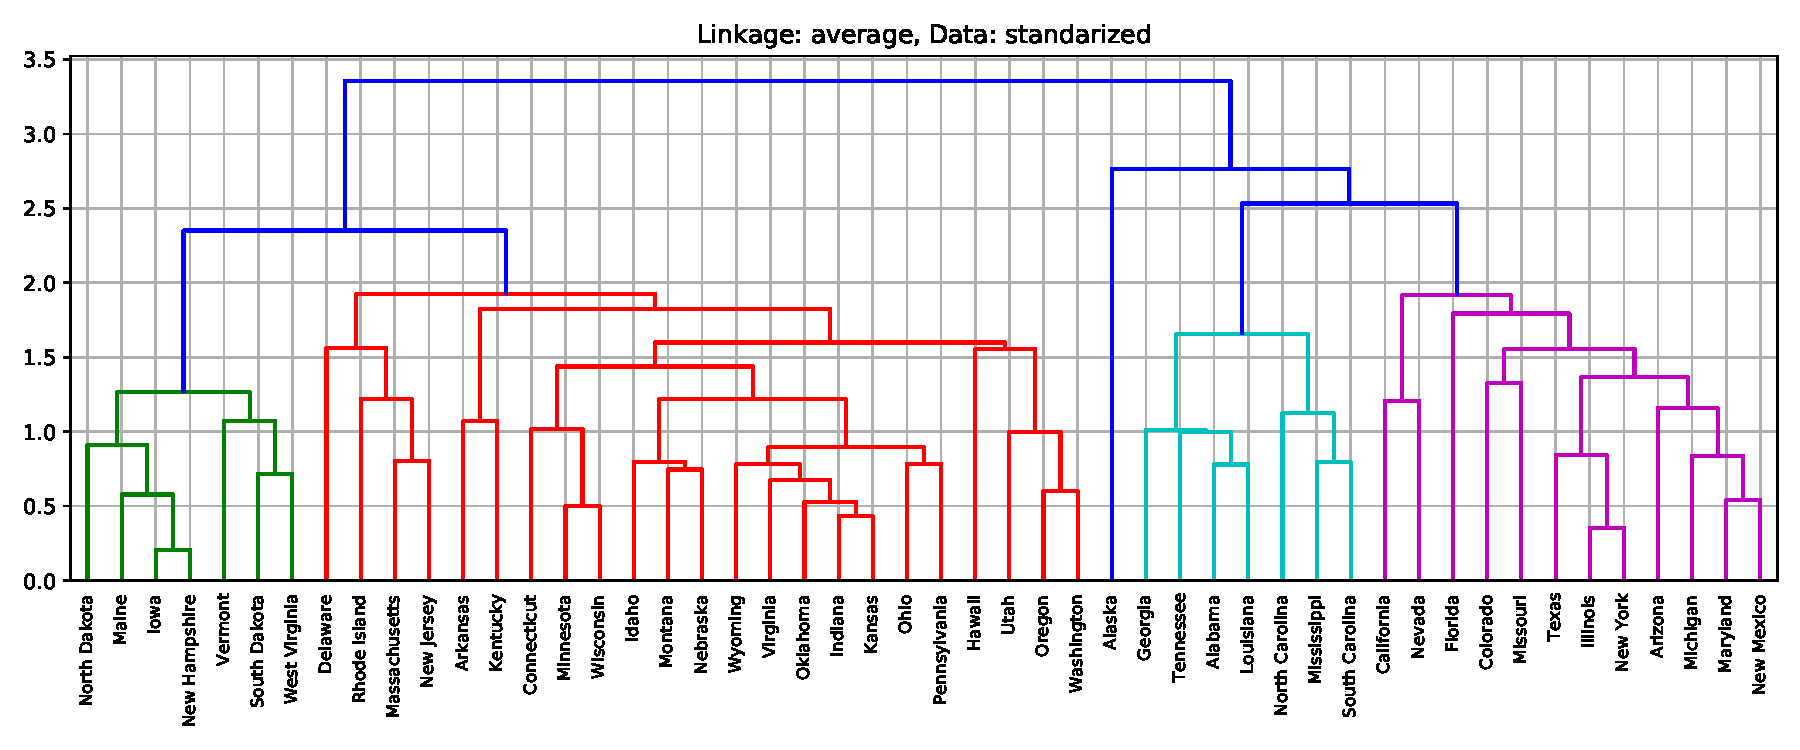
\includegraphics[width = 0.90\textwidth]{2-averagestandarized.pdf}
    \caption{Clustering para datos estandarizados con enlace completo}
    \label{2-averagestandarized}
\end{figure}
\begin{figure}[H]
    \centering
    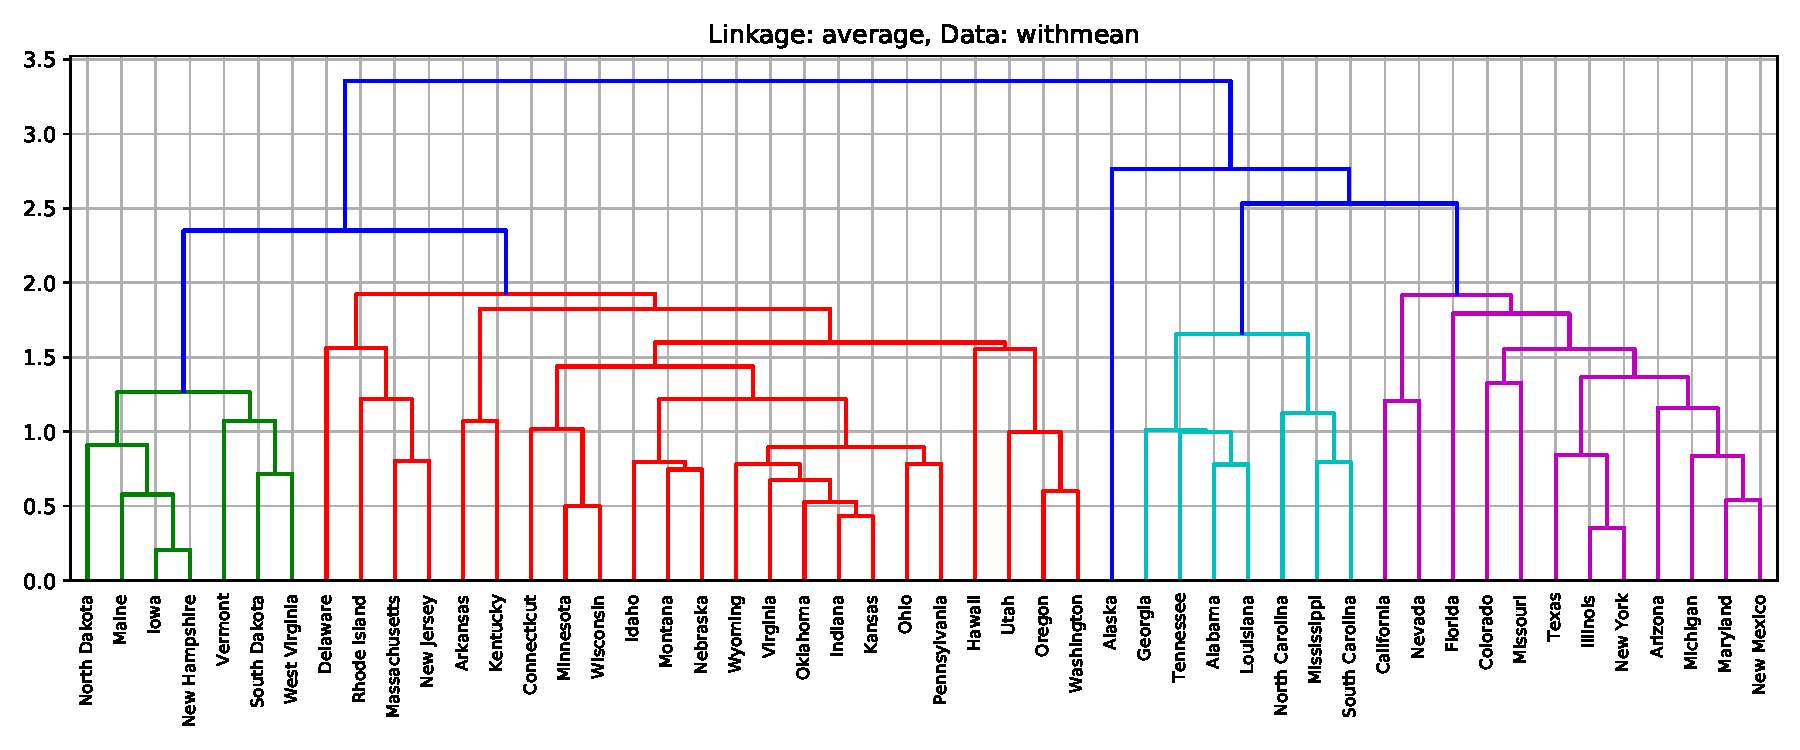
\includegraphics[width = 0.90\textwidth]{2-averagewithmean.pdf}
    \caption{Clustering para datos con $\sigma^2 = 1$ con enlace completo}
    \label{2-averagewithmean}
\end{figure}
\subsection*{Resultados del clustering con $K$-means para el ejercicio 10}
\begin{figure}[H]
    \centering
    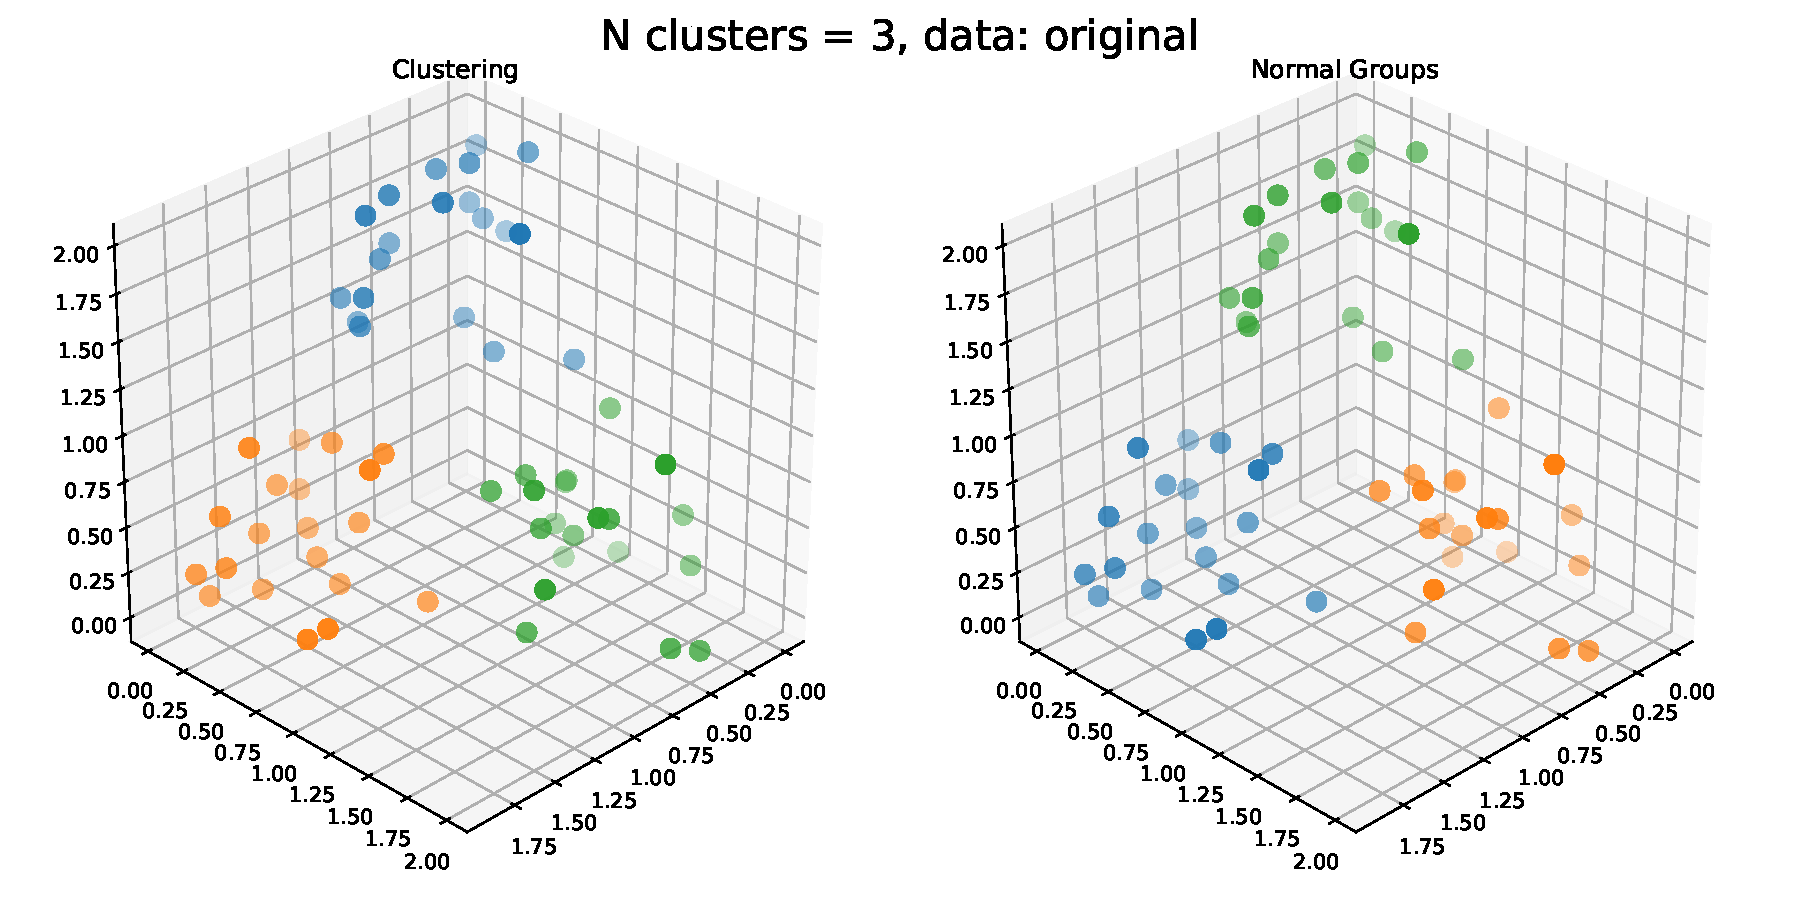
\includegraphics[width = 0.75\textwidth]{3-original-3.pdf}
    \caption{Clustering para datos originales con $K =3$}
    \label{3-original-3}
\end{figure}
\begin{figure}[H]
    \centering
    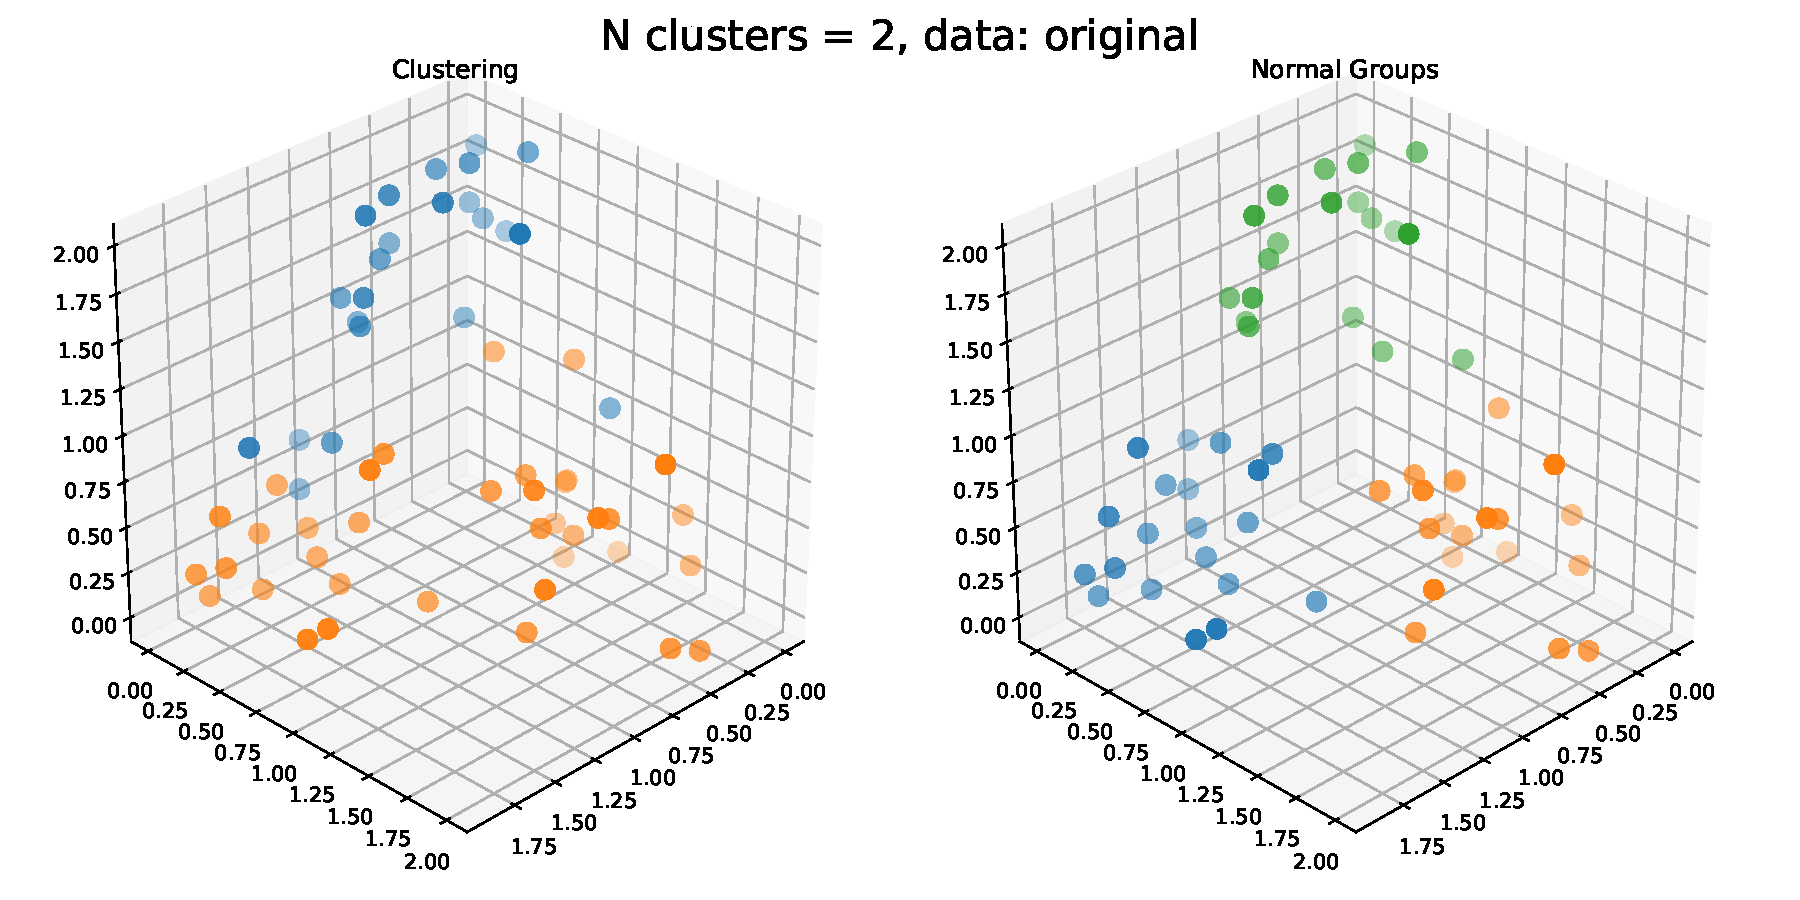
\includegraphics[width = 0.75\textwidth]{3-original-2.pdf}
    \caption{Clustering para datos originales con $K =2$}
    \label{3-original-2}
\end{figure}
\begin{figure}[H]
    \centering
    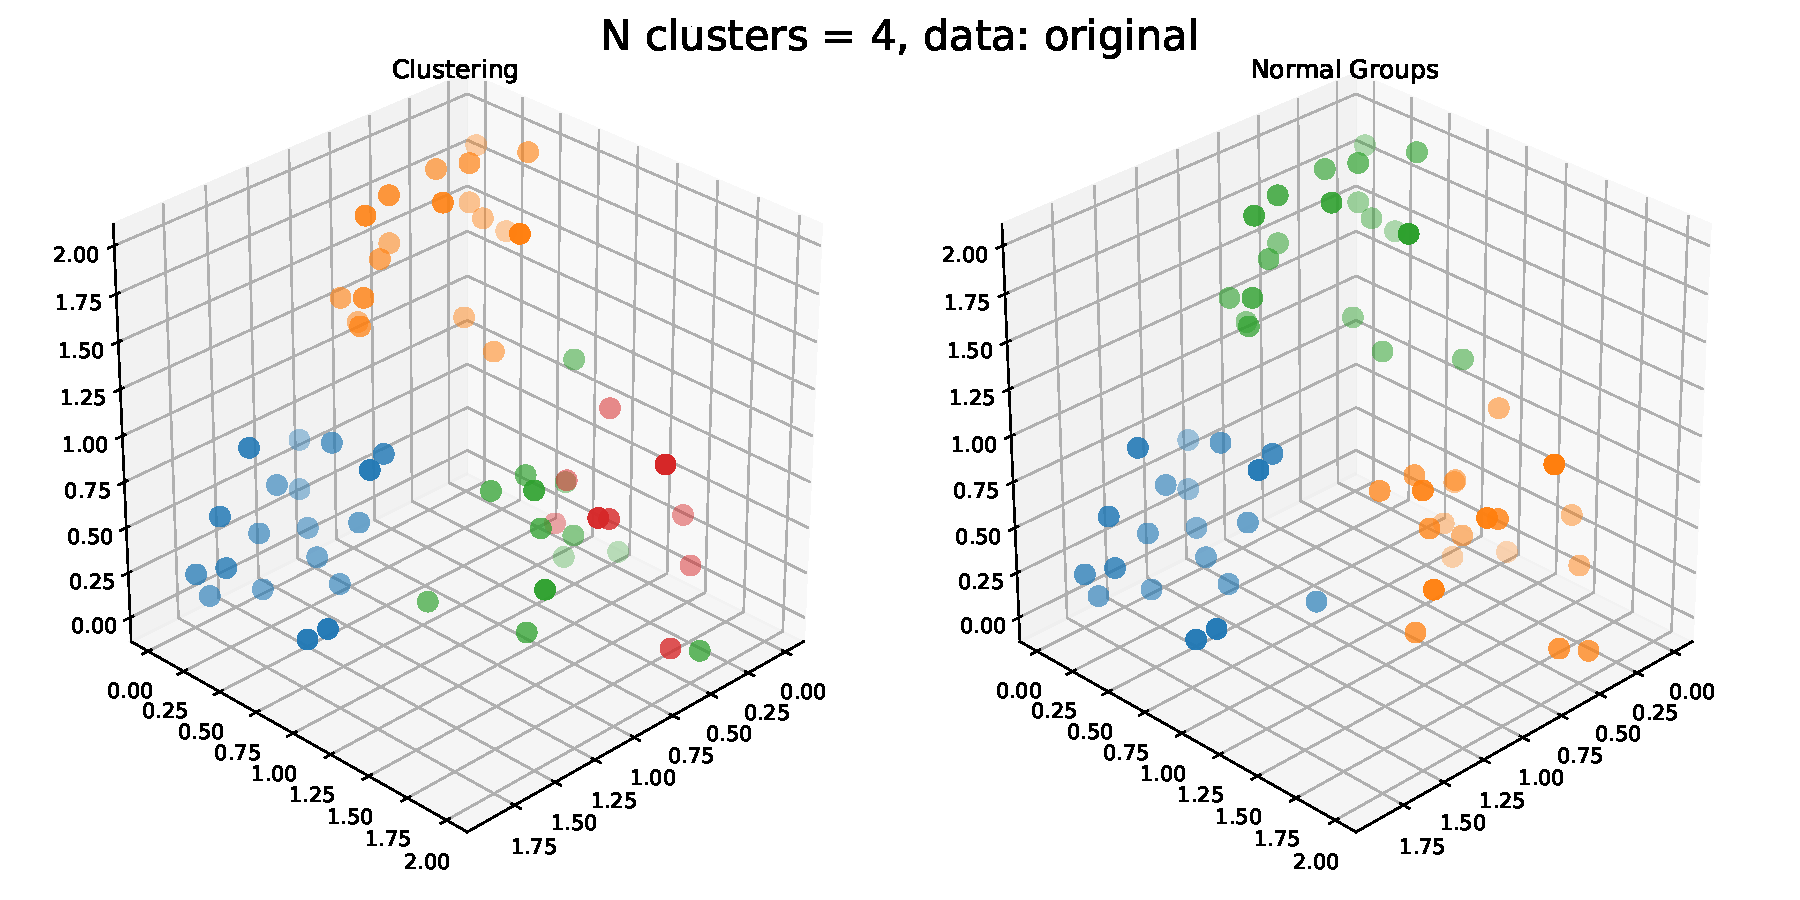
\includegraphics[width = 0.75\textwidth]{3-original-4.pdf}
    \caption{Clustering para datos originales con $K =4$}
    \label{3-original-4}
\end{figure}
\begin{figure}[H]
    \centering
    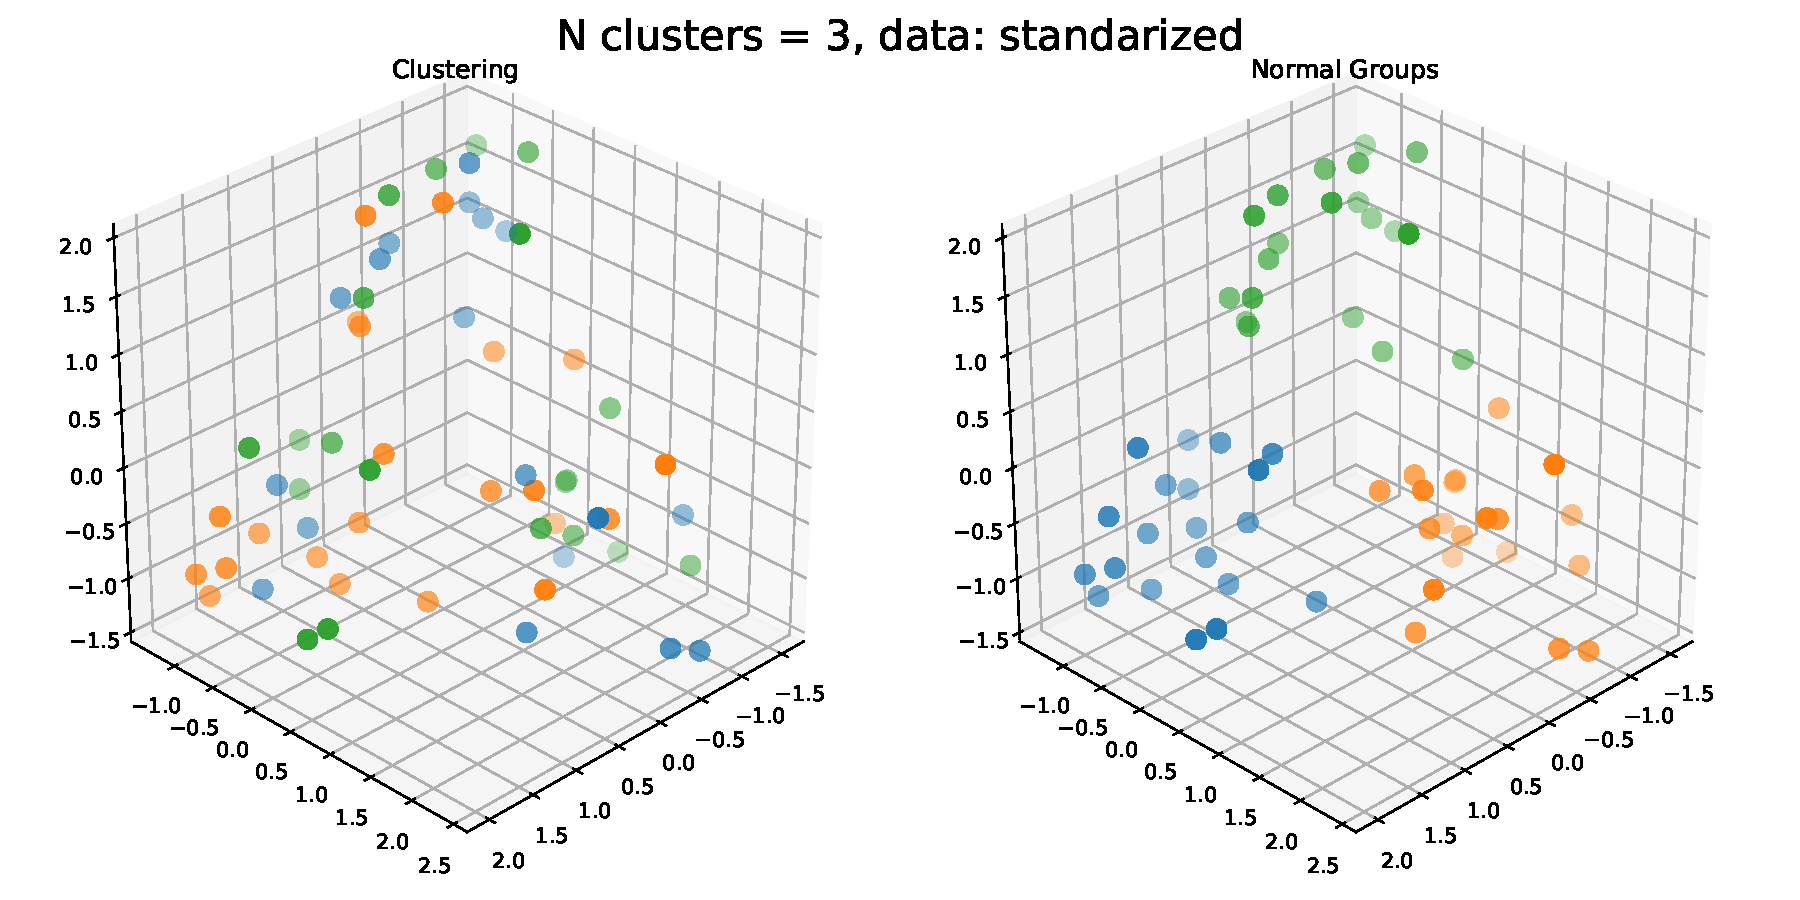
\includegraphics[width = 0.75\textwidth]{3-standarized-3.pdf}
    \caption{Clustering para datos estandarizados con $K = 3$}
    \label{3-standarized-3}
\end{figure}
\begin{figure}[H]
    \centering
    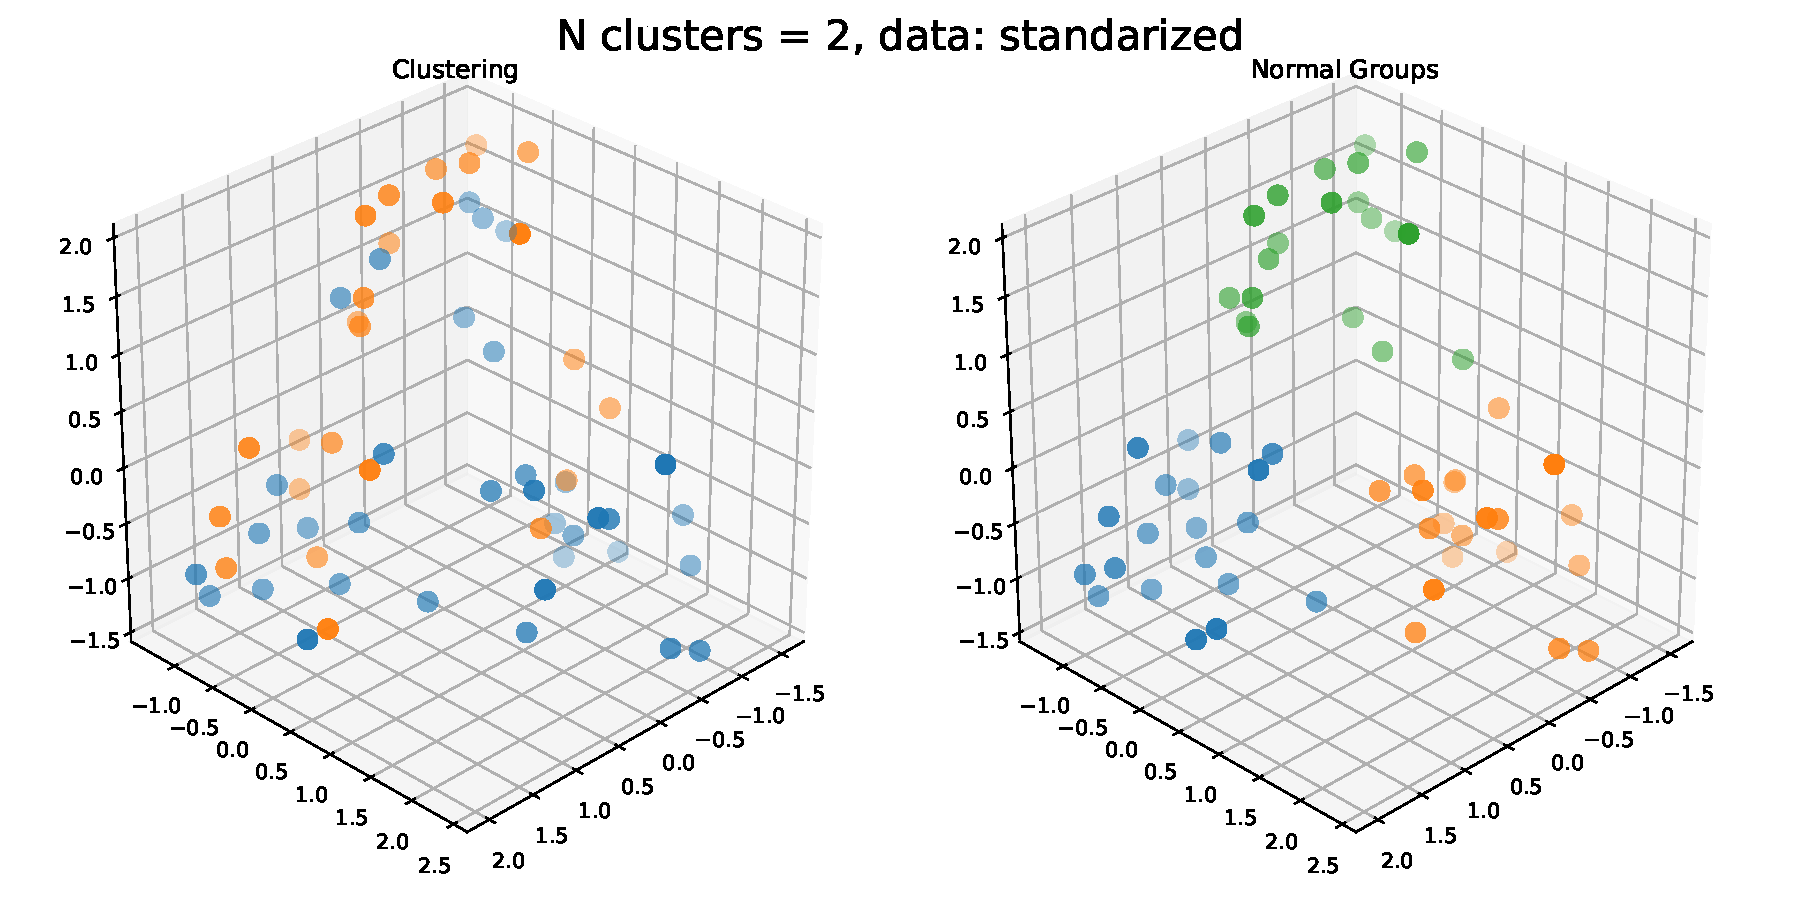
\includegraphics[width = 0.75\textwidth]{3-standarized-2.pdf}
    \caption{Clustering para datos estandarizados con $K = 2$}
    \label{3-standarized-2}
\end{figure}
\begin{figure}[H]
    \centering
    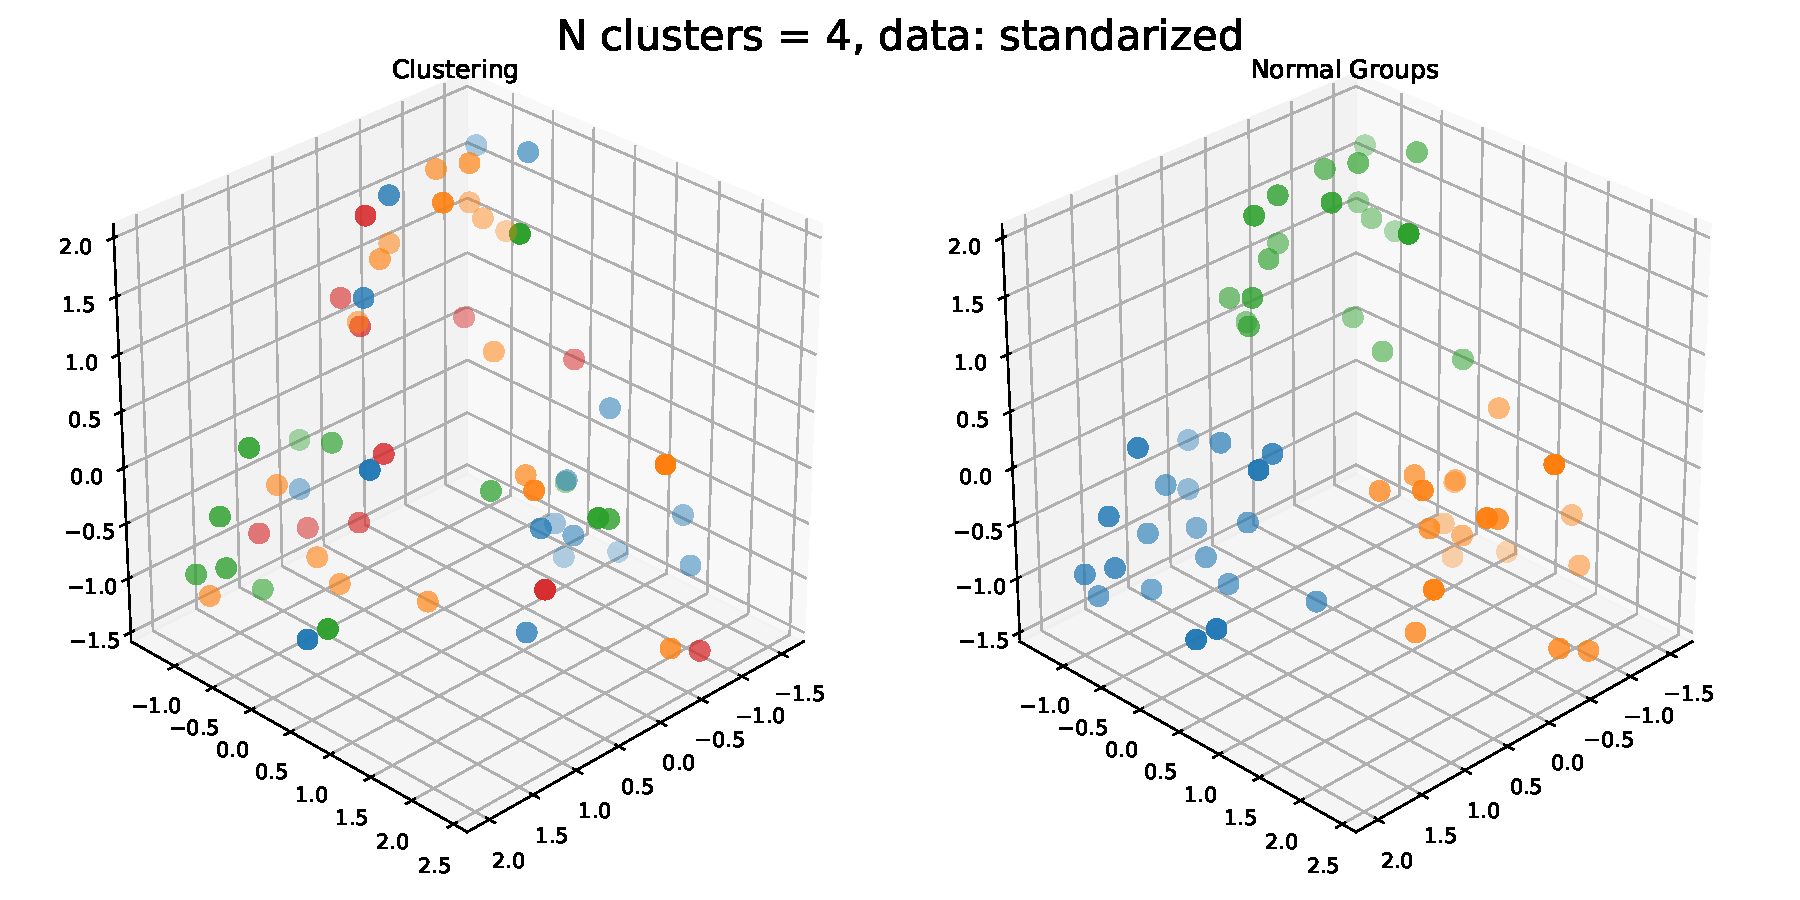
\includegraphics[width = 0.75\textwidth]{3-standarized-4.pdf}
    \caption{Clustering para datos estandarizados con $K = 4$}
    \label{3-standarized-4}
\end{figure}
\begin{figure}[H]
    \centering
    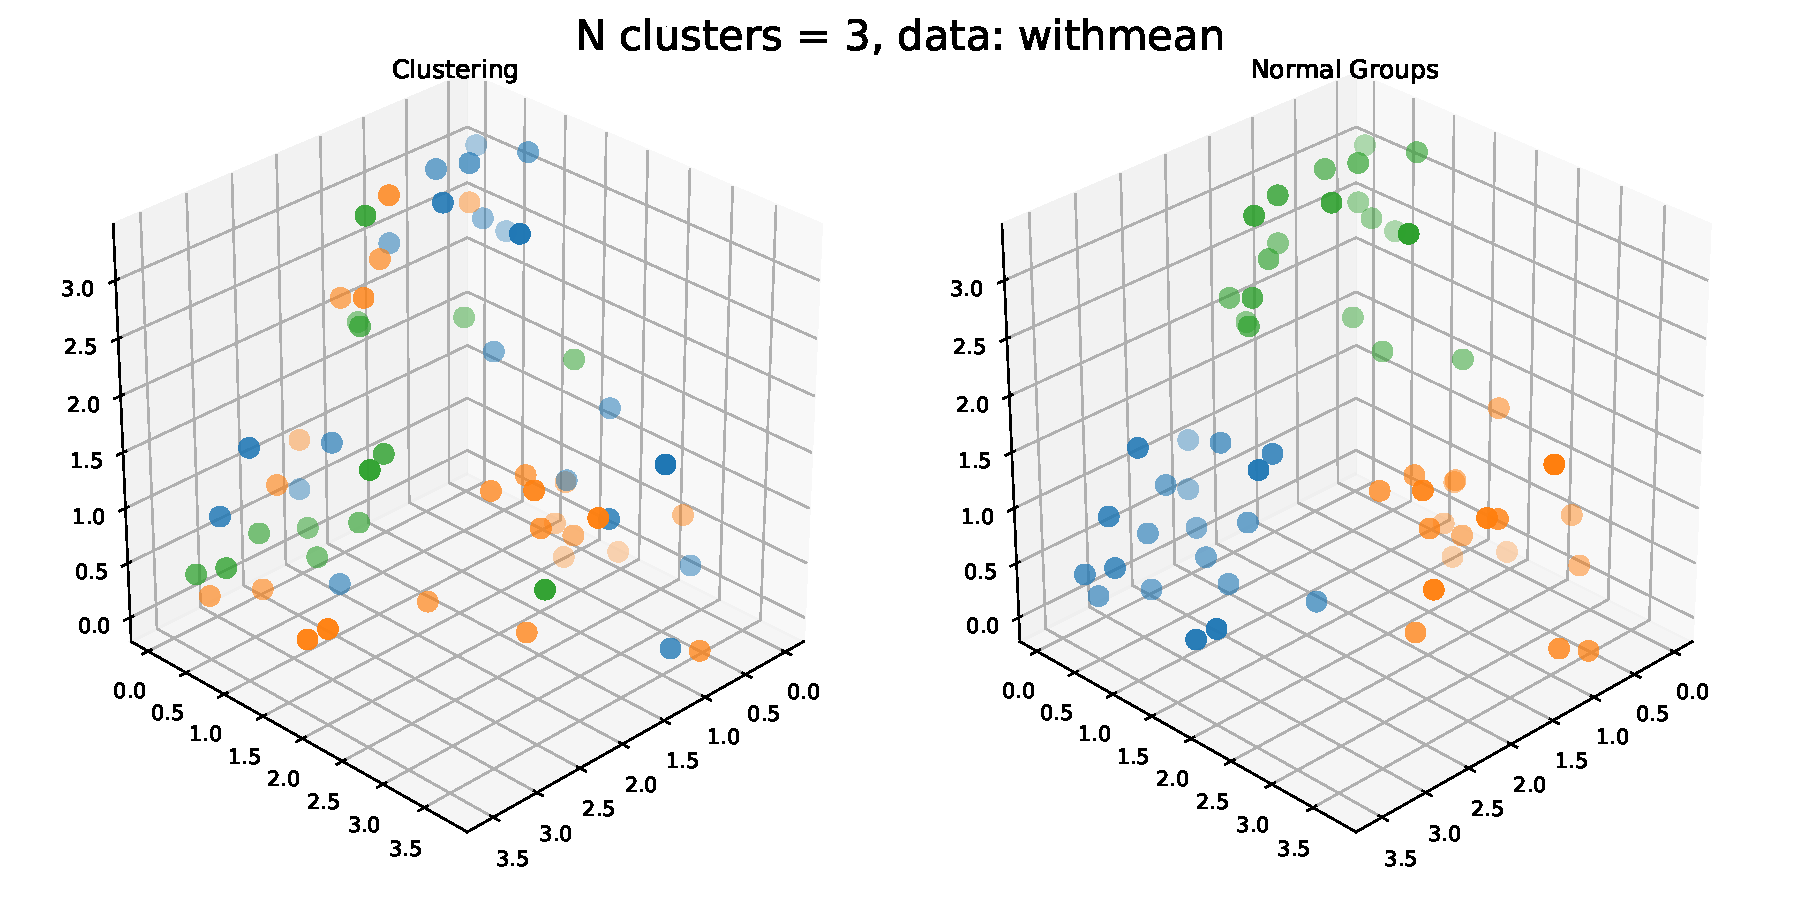
\includegraphics[width = 0.75\textwidth]{3-withmean-3.pdf}
    \caption{Clustering para datos con $\sigma^2=1$ con $K = 3$}
    \label{3-withmean-3}
\end{figure}
\begin{figure}[H]
    \centering
    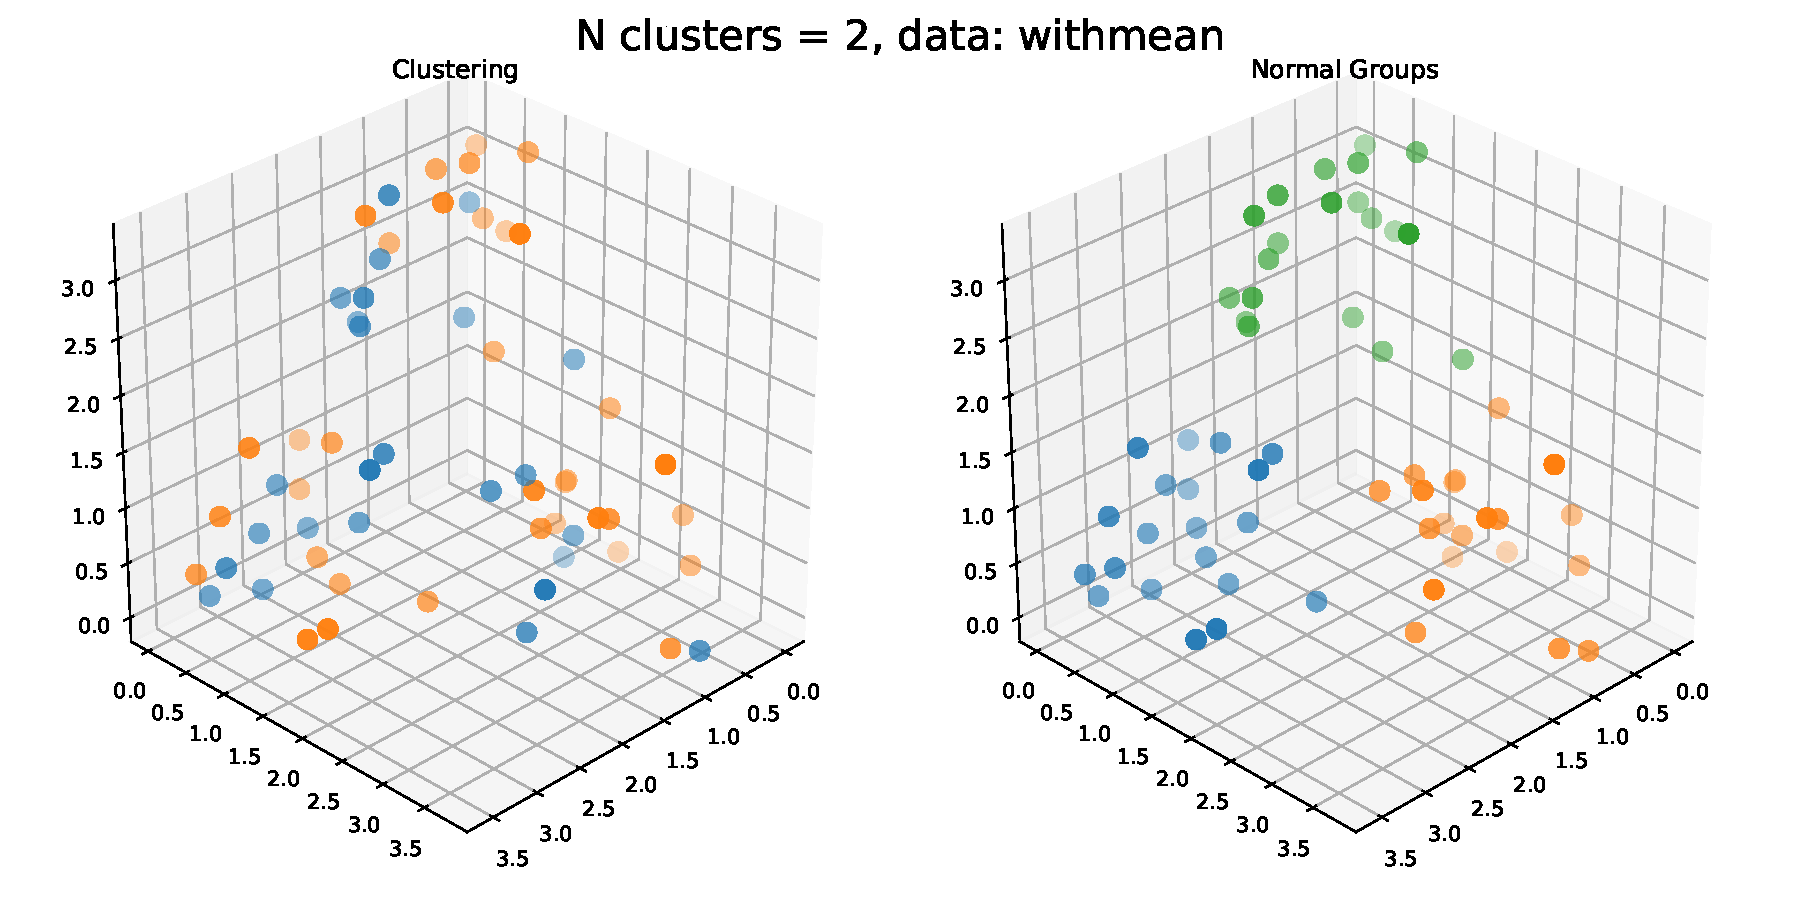
\includegraphics[width = 0.75\textwidth]{3-withmean-2.pdf}
    \caption{Clustering para datos con $\sigma^2=1$ con $K = 2$}
    \label{3-withmean-2}
\end{figure}
\begin{figure}[H]
    \centering
    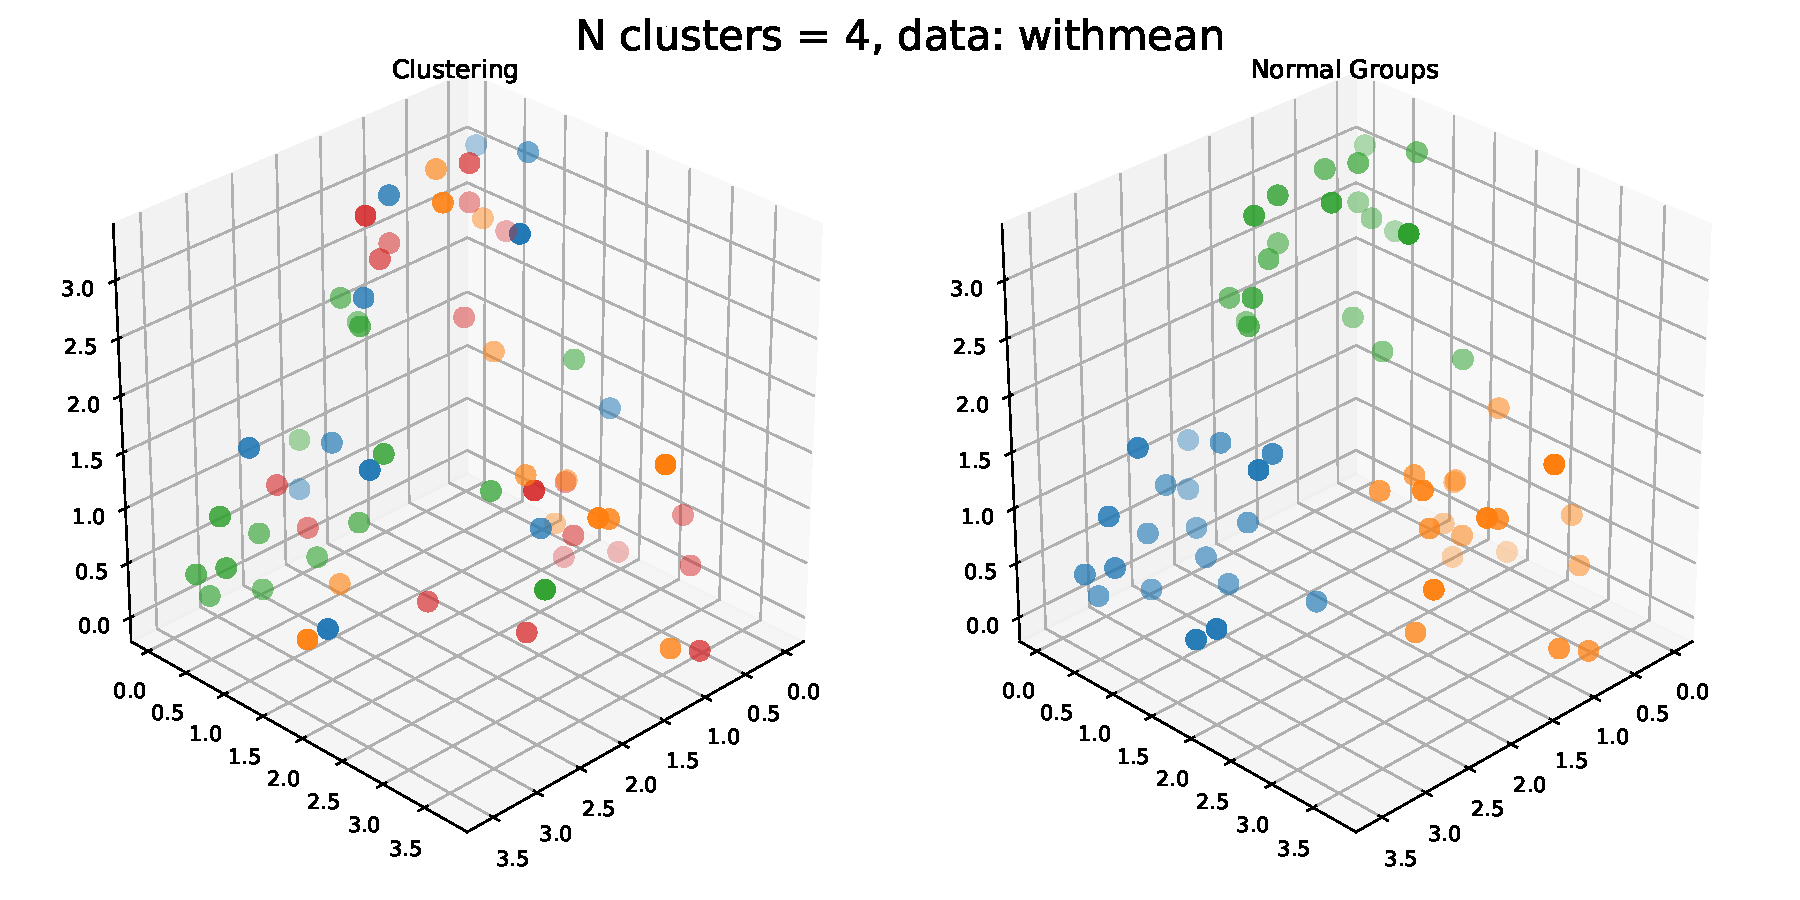
\includegraphics[width = 0.75\textwidth]{3-withmean-4.pdf}
    \caption{Clustering para datos con $\sigma^2=1$ con $K = 4$}
    \label{3-withmean-4}
\end{figure}
\begin{figure}[H]
    \centering
    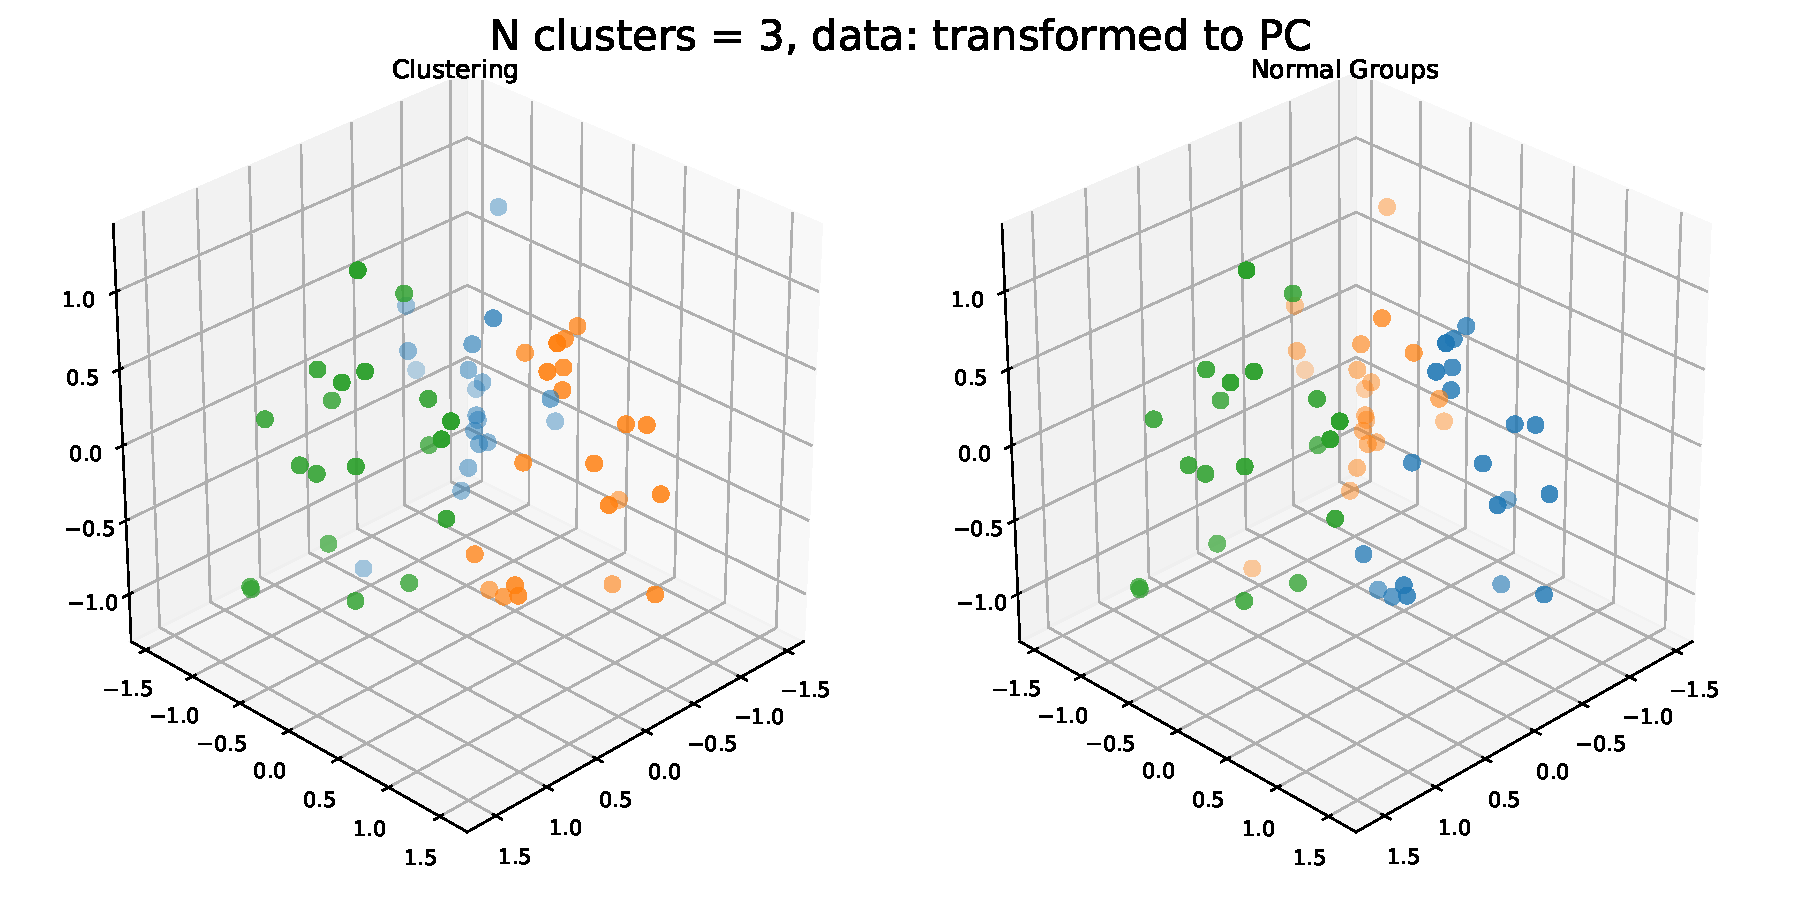
\includegraphics[width = 0.75\textwidth]{3-2pcs-3.pdf}
    \caption{Clustering sobre las primeras dos componentes principales con $K = 3$}
    \label{3-2pcs-3}
\end{figure}
\begin{figure}[H]
    \centering
    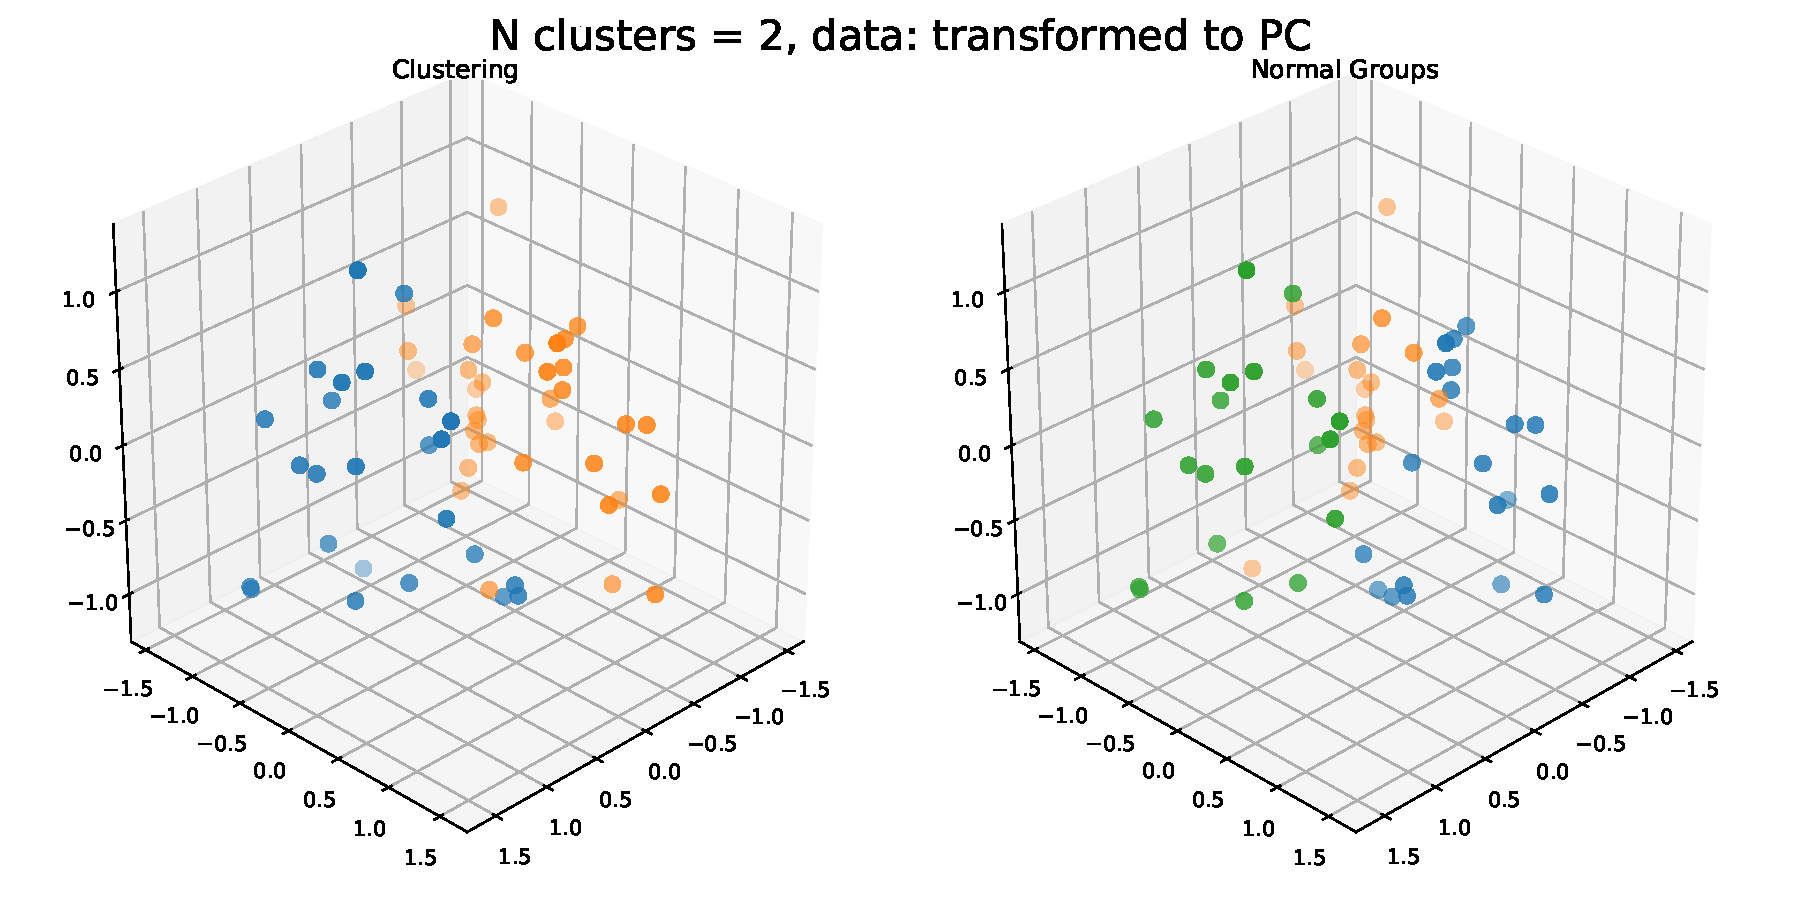
\includegraphics[width = 0.75\textwidth]{3-2pcs-2.pdf}
    \caption{Clustering sobre las primeras dos componentes principales con $K = 2$}
    \label{3-2pcs-2}
\end{figure}
\begin{figure}[H]
    \centering
    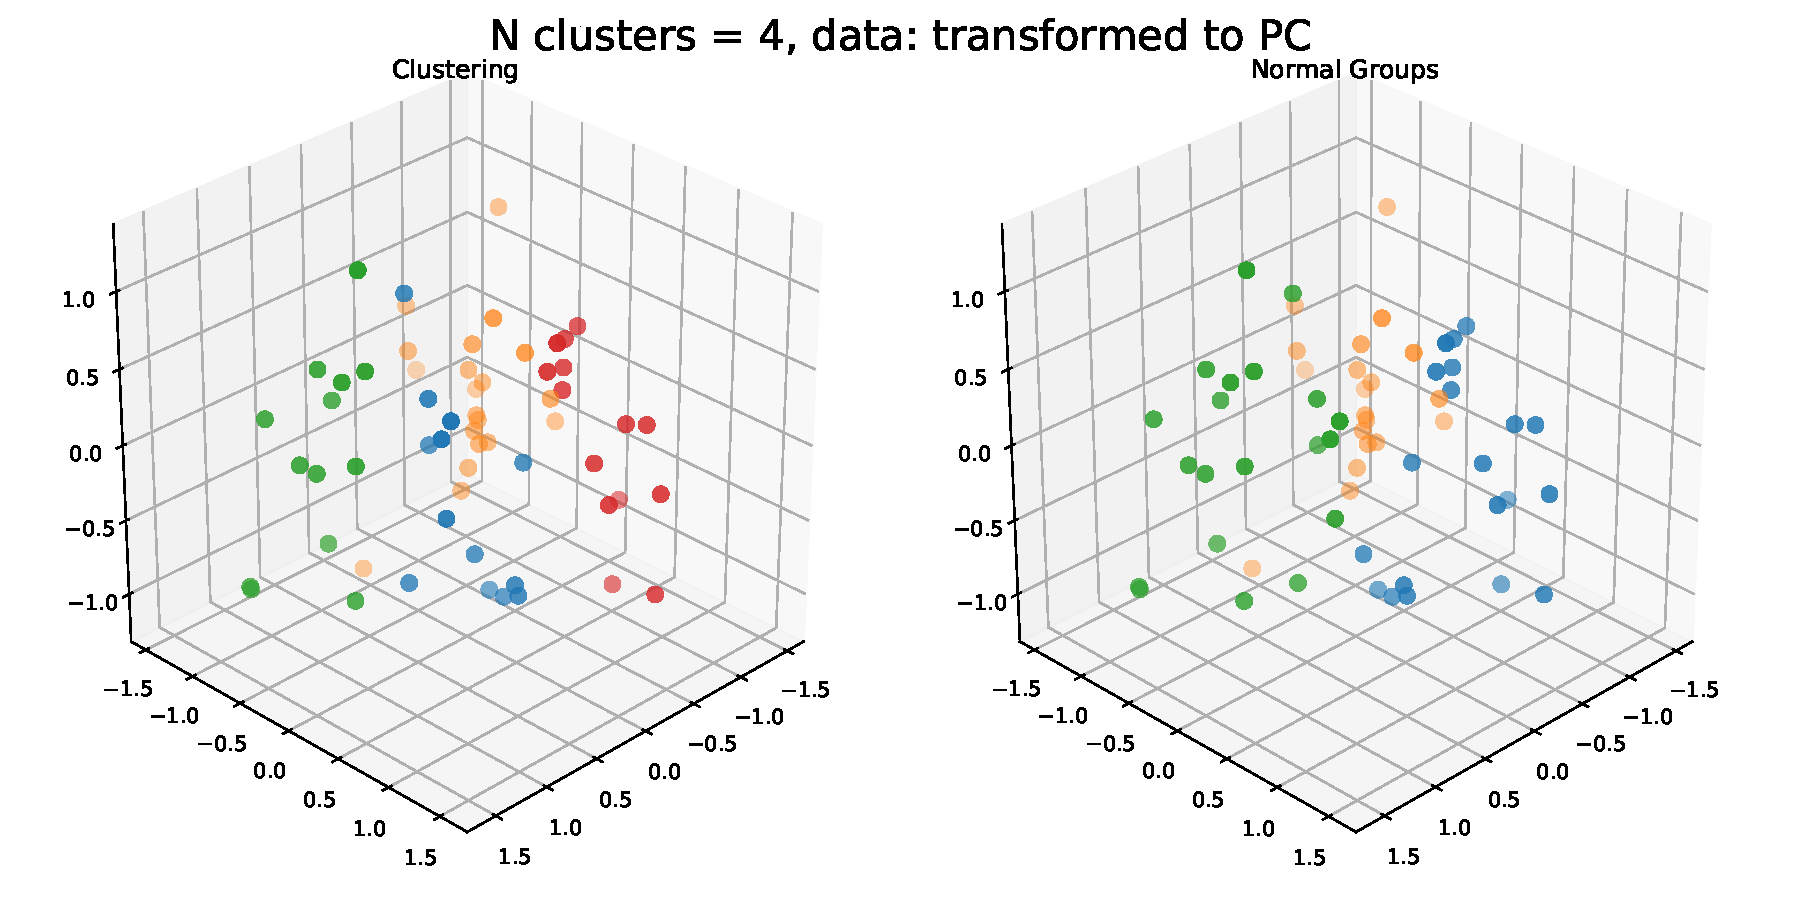
\includegraphics[width = 0.75\textwidth]{3-2pcs-4.pdf}
    \caption{Clustering sobre las primeras dos componentes principales con $K = 4$}
    \label{3-2pcs-4}
\end{figure}
\subsection*{Dendogramas para el ejercicio 11}
\begin{figure}[H]
    \centering
    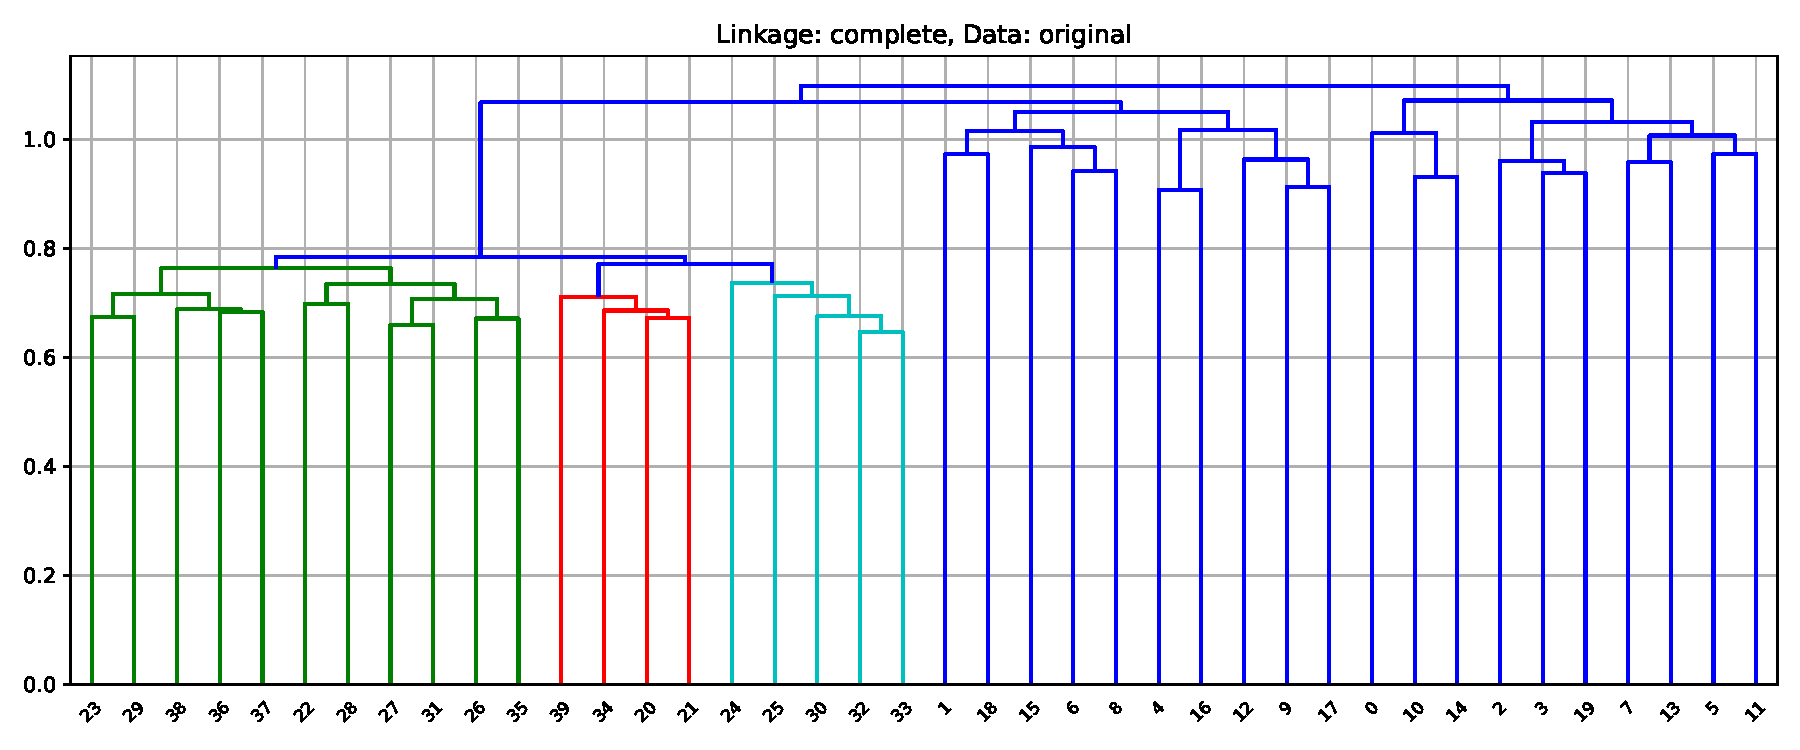
\includegraphics[width = 0.90\textwidth]{4-completeoriginal.pdf}
    \caption{Clustering para datos originales con enlace completo}
    \label{4-completeoriginal}
\end{figure}
\begin{figure}[H]
    \centering
    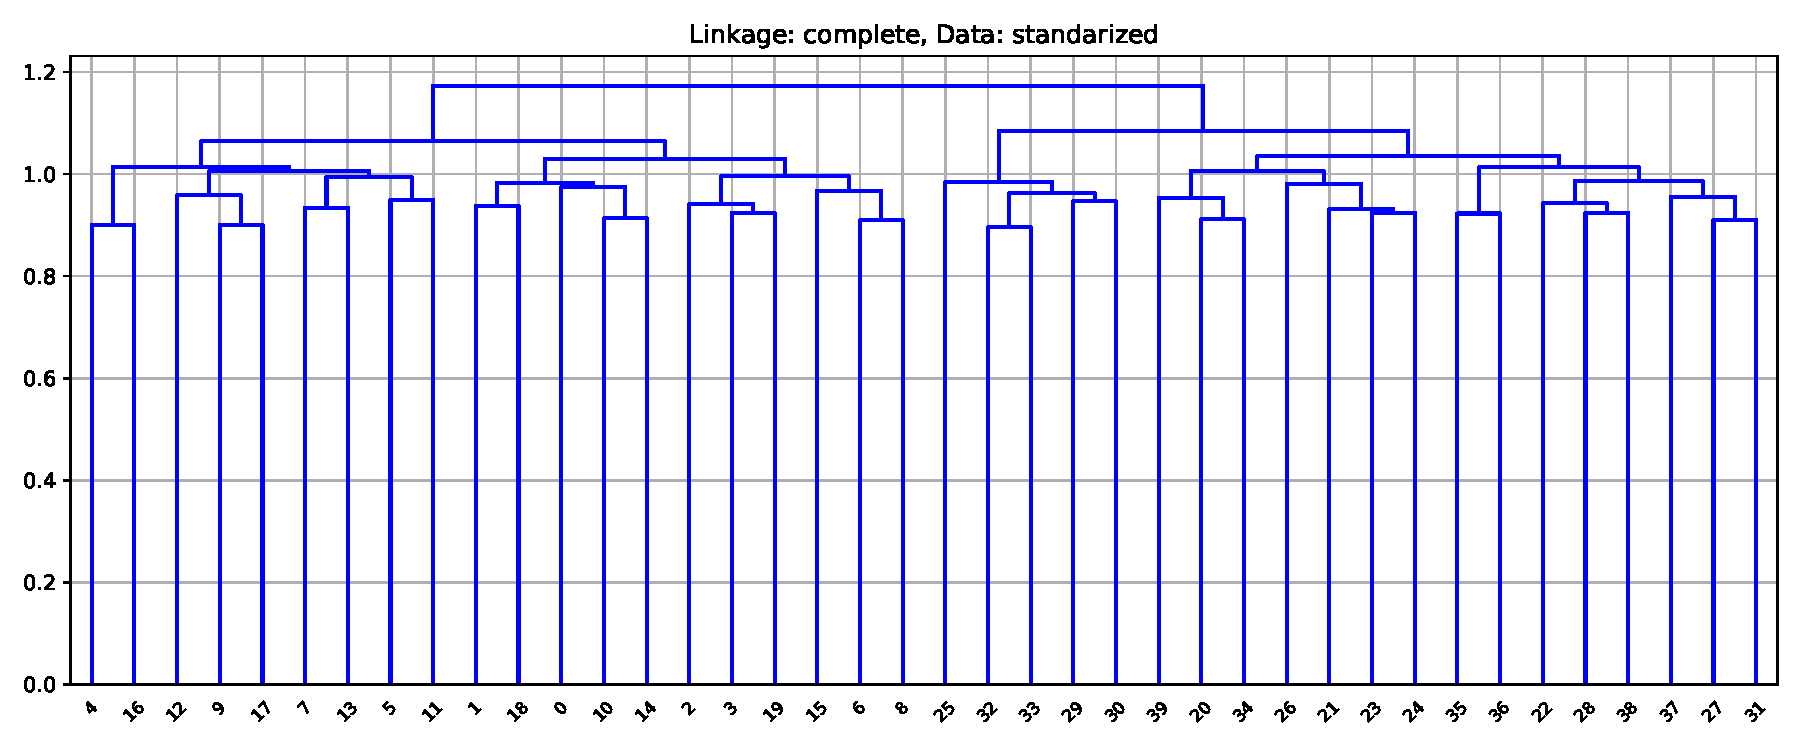
\includegraphics[width = 0.90\textwidth]{4-completestandarized.pdf}
    \caption{Clustering para datos estandarizados con enlace completo}
    \label{4-completestandarized}
\end{figure}
\begin{figure}[H]
    \centering
    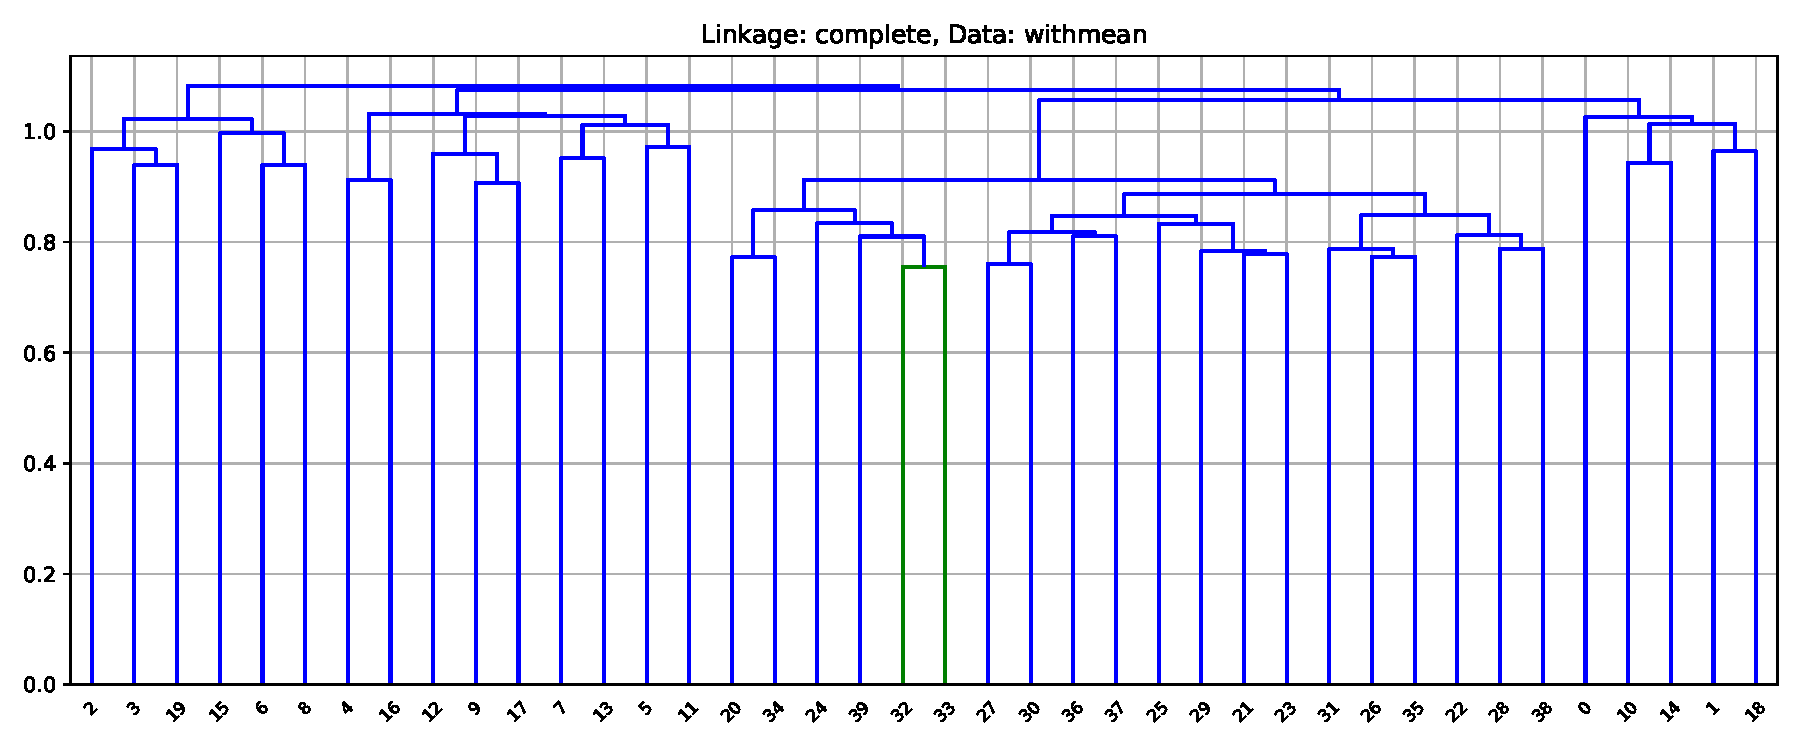
\includegraphics[width = 0.90\textwidth]{4-completewithmean.pdf}
    \caption{Clustering para datos con $\sigma^2 = 1$ con enlace completo}
    \label{4-completewithmean}
\end{figure}
\begin{figure}[H]
    \centering
    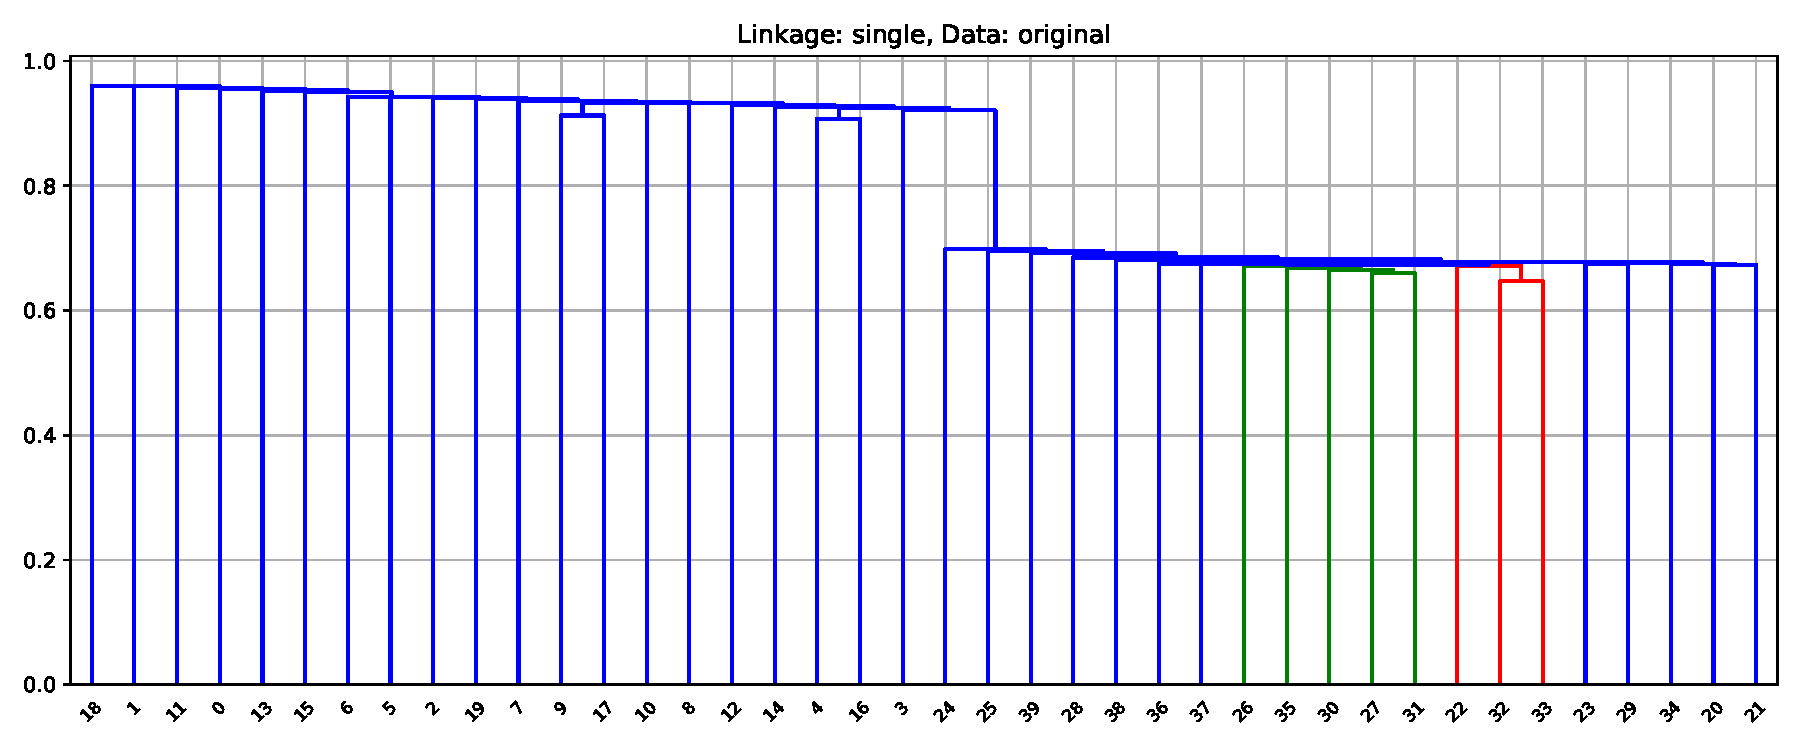
\includegraphics[width = 0.90\textwidth]{4-singleoriginal.pdf}
    \caption{Clustering para datos originales con enlace completo}
    \label{4-singleoriginal}
\end{figure}
\begin{figure}[H]
    \centering
    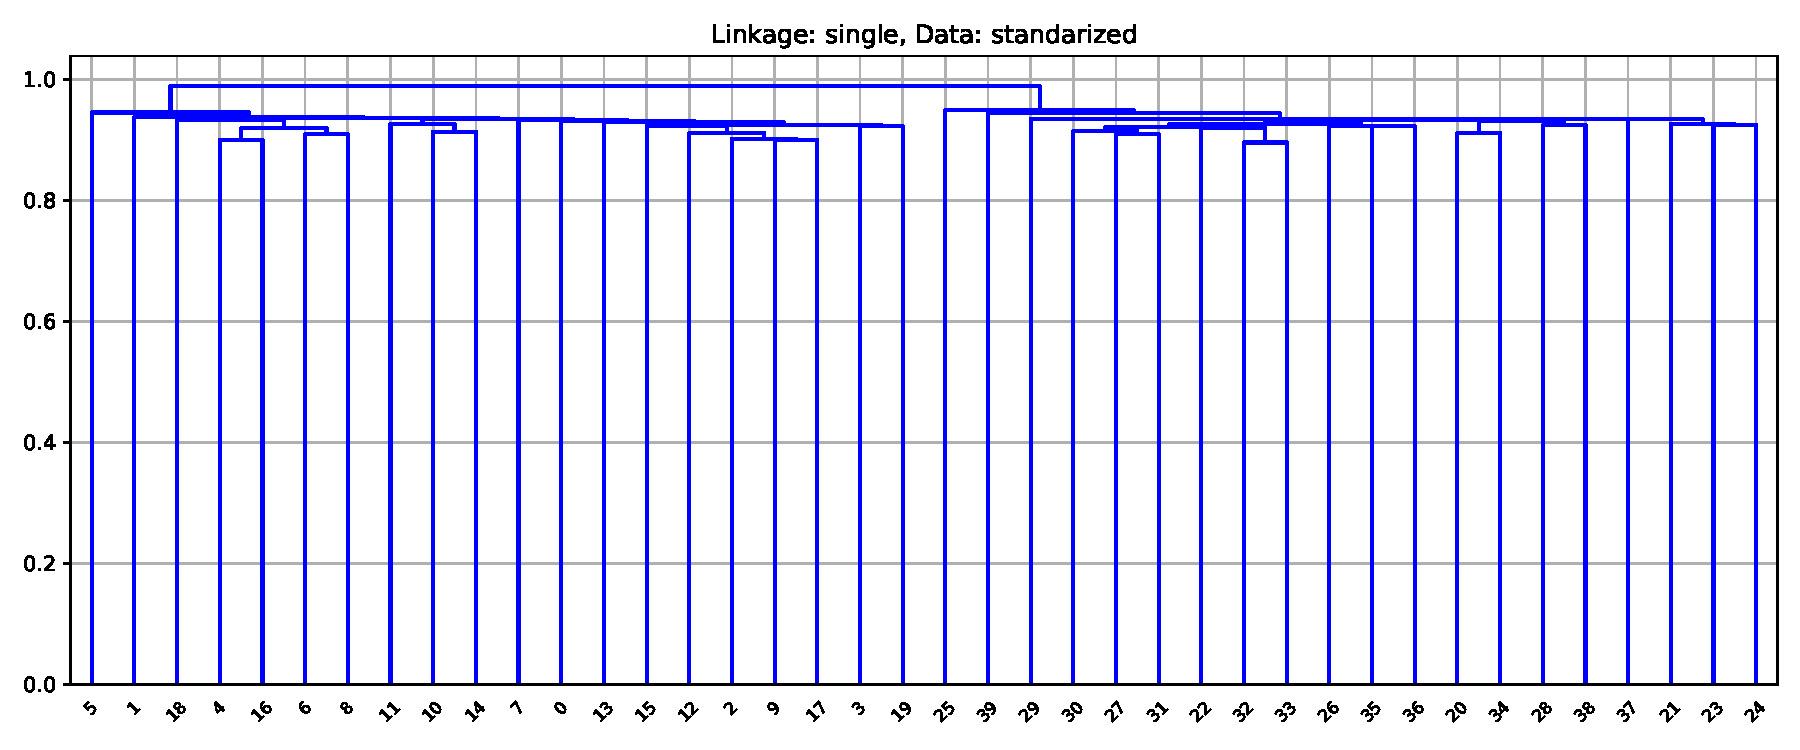
\includegraphics[width = 0.90\textwidth]{4-singlestandarized.pdf}
    \caption{Clustering para datos estandarizados con enlace completo}
    \label{4-singlestandarized}
\end{figure}
\begin{figure}[H]
    \centering
    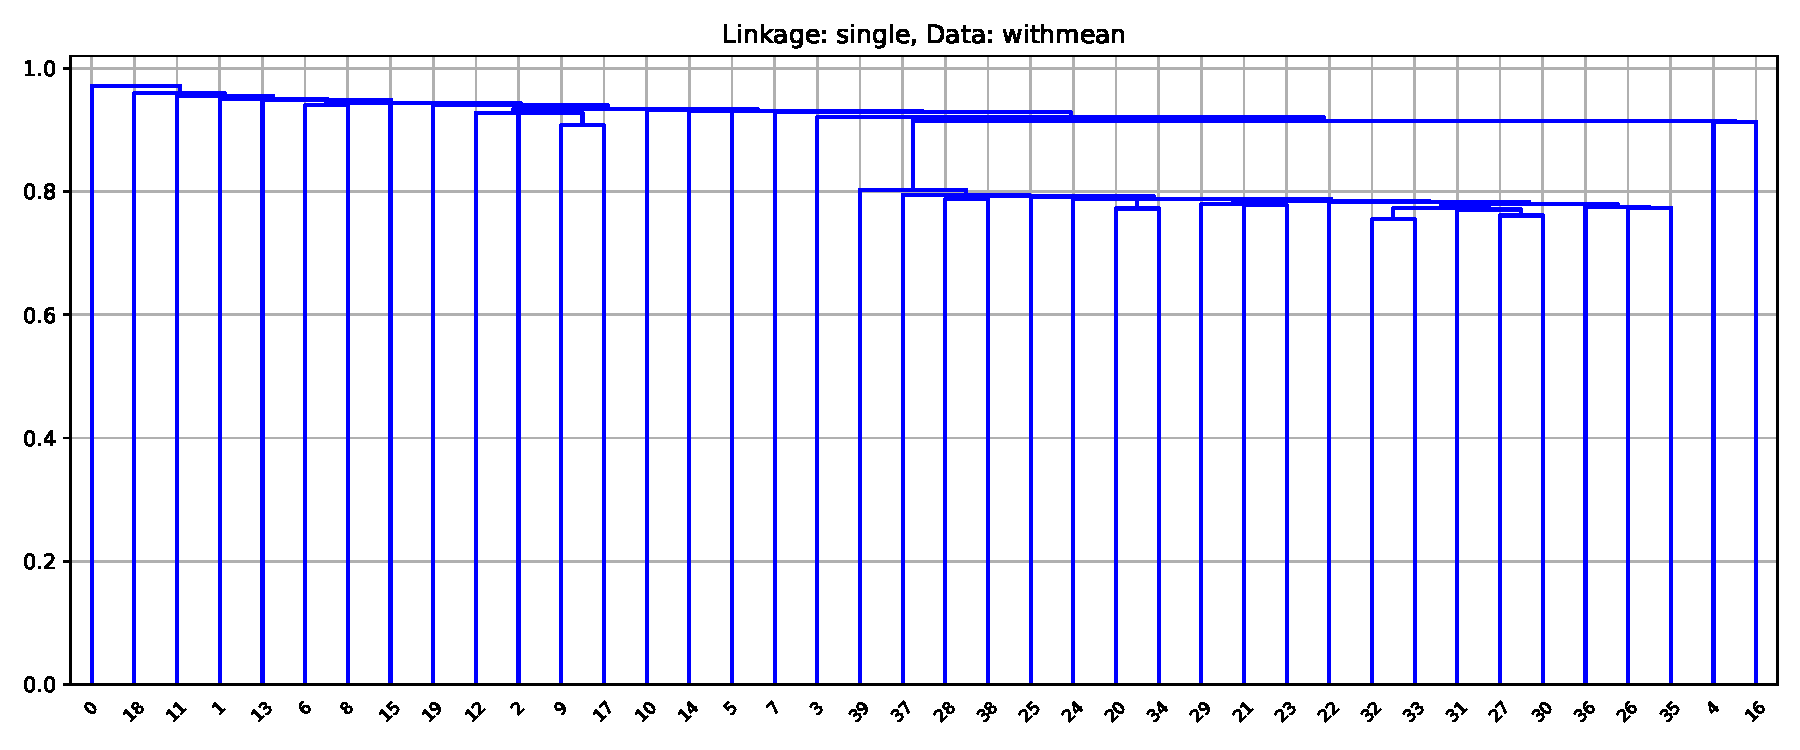
\includegraphics[width = 0.90\textwidth]{4-singlewithmean.pdf}
    \caption{Clustering para datos con $\sigma^2 = 1$ con enlace completo}
    \label{4-singlewithmean}
\end{figure}
\begin{figure}[H]
    \centering
    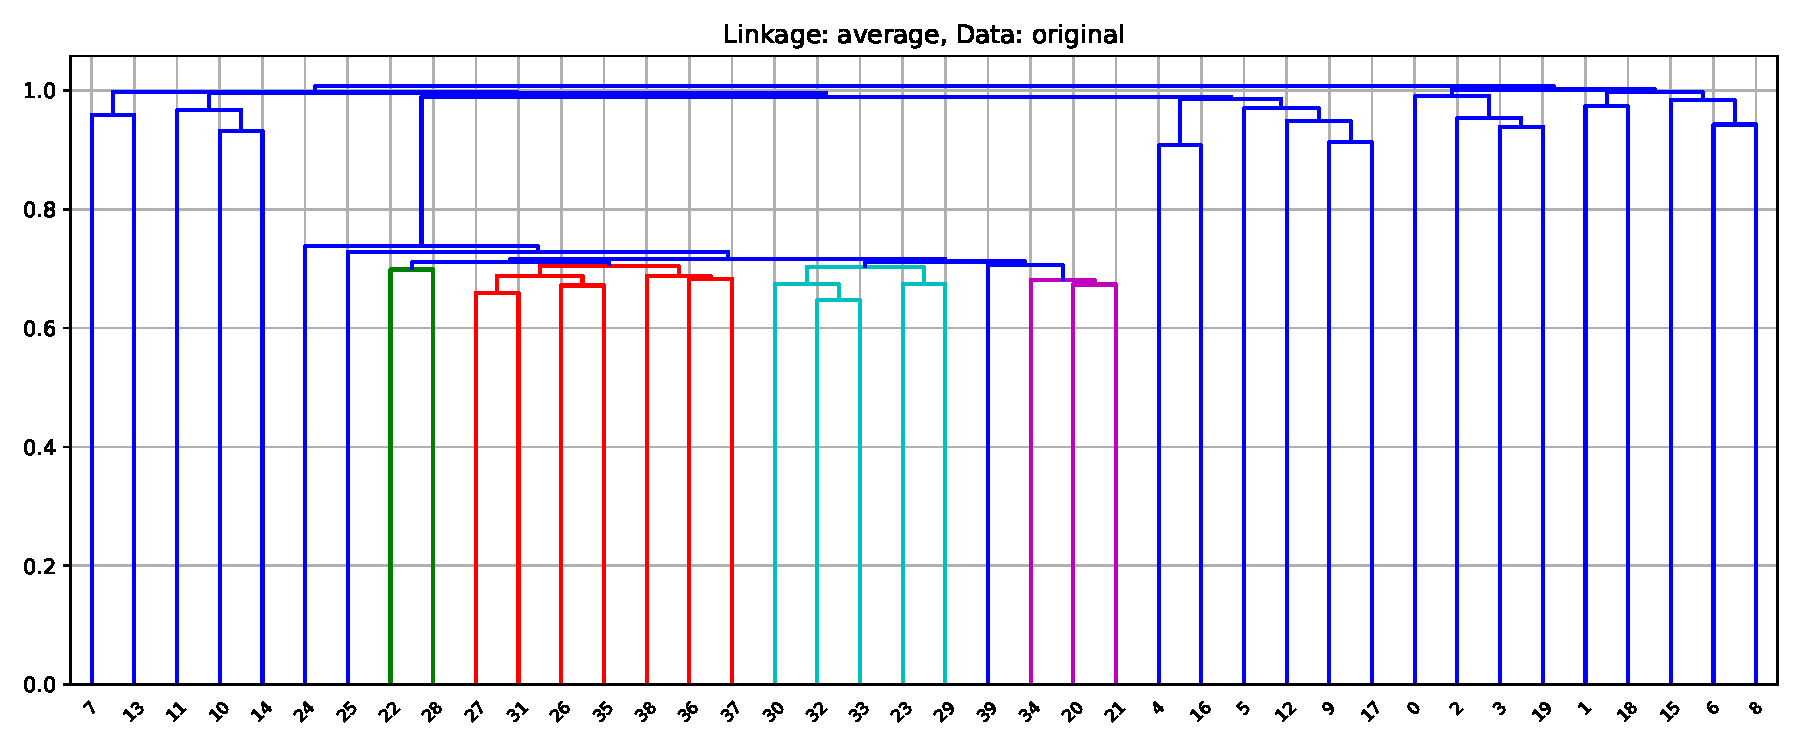
\includegraphics[width = 0.90\textwidth]{4-averageoriginal.pdf}
    \caption{Clustering para datos originales con enlace completo}
    \label{4-averageoriginal}
\end{figure}
\begin{figure}[H]
    \centering
    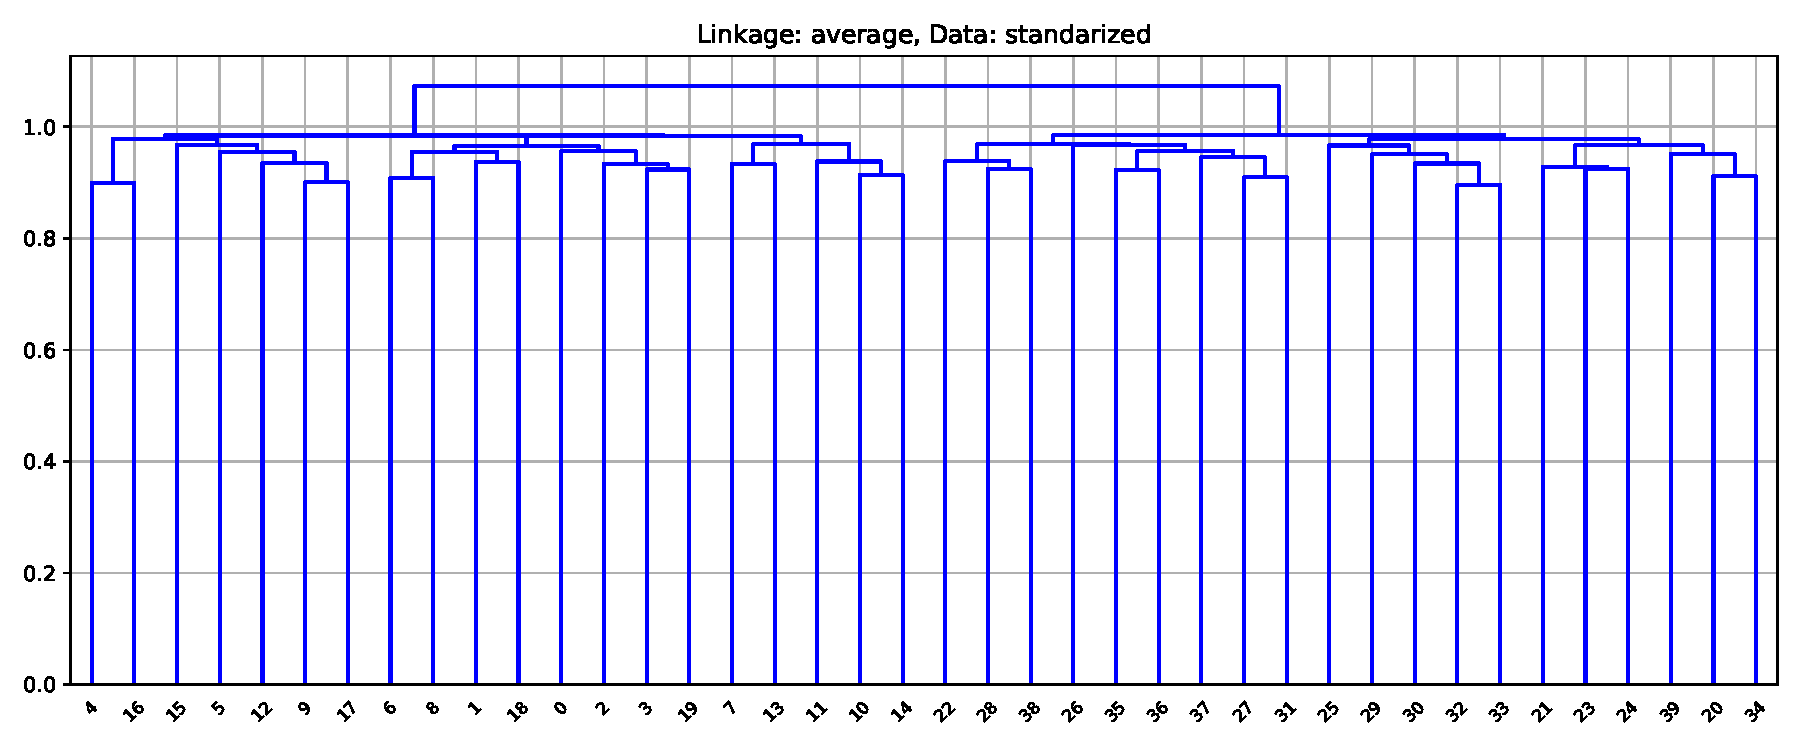
\includegraphics[width = 0.90\textwidth]{4-averagestandarized.pdf}
    \caption{Clustering para datos estandarizados con enlace completo}
    \label{4-averagestandarized}
\end{figure}
\begin{figure}[H]
    \centering
    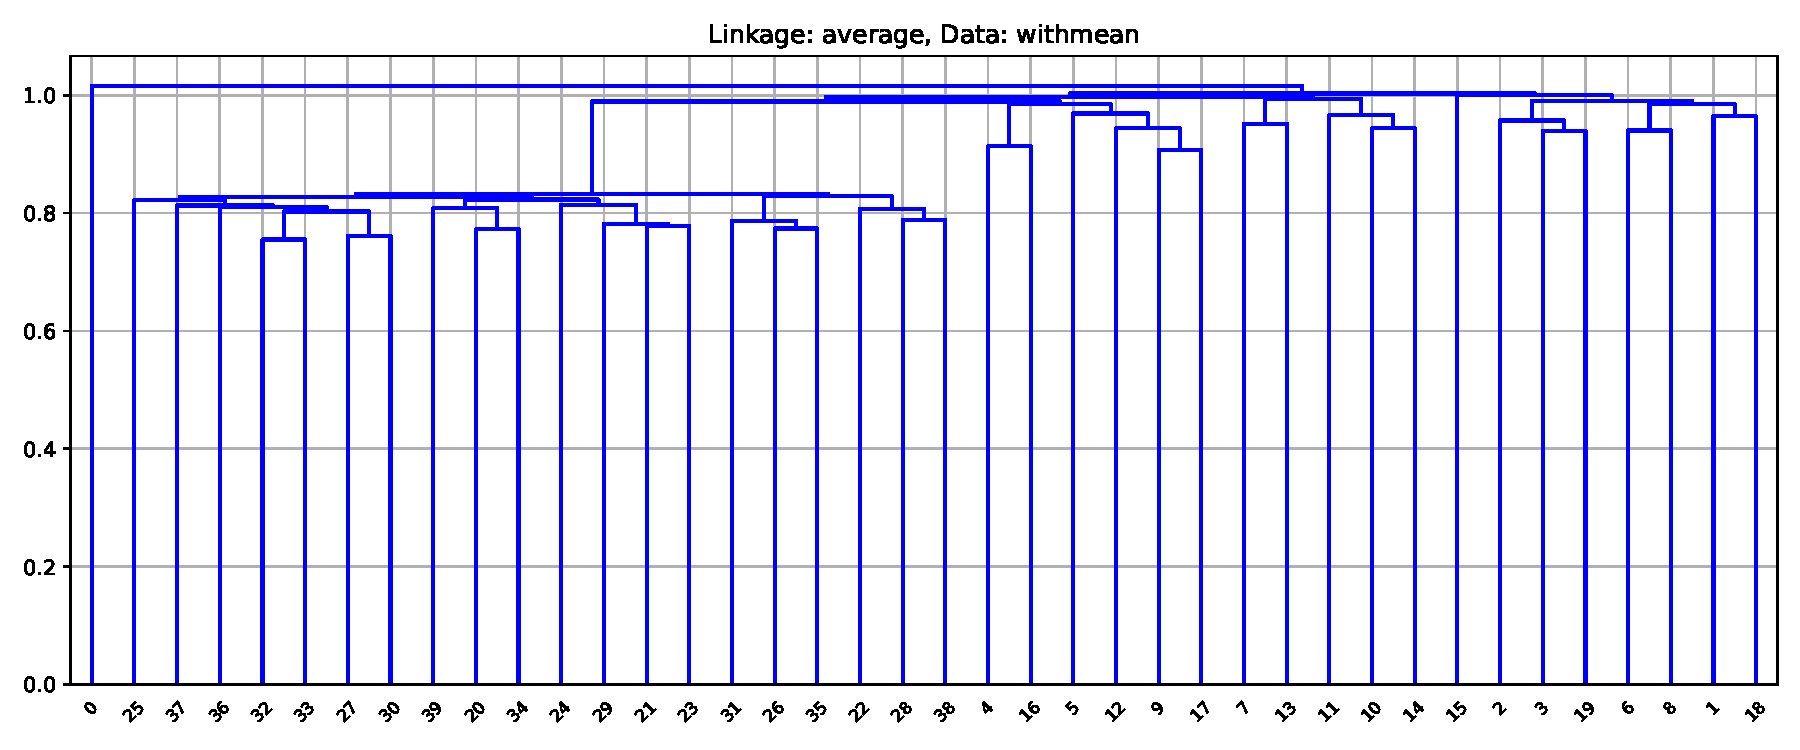
\includegraphics[width = 0.90\textwidth]{4-averagewithmean.pdf}
    \caption{Clustering para datos con $\sigma^2 = 1$ con enlace completo}
    \label{4-averagewithmean}
\end{figure}

\pagebreak
\section*{Anexo 3: código en Python de los problemas}
\lstinputlisting[language=Python]{tarea2.py}
\begin{thebibliography}{9}
    \bibitem{isl} Hastie et al. \textit{An Introduction to Statitistical Learning}. Editorial Springer.  Séptima edición. 2013.
\end{thebibliography}
\end{document}